\appendix
\section{M0 Experimental Design}
\subsection{Opaque catalogs}
The generator in \texttt{src/data/agent\_resources.py} creates identifiers such
as \texttt{tool\_zaf\_193}. Each resource combines held-out action, object, and
family concepts with aliases, a schema, a version, and a side-effect class.
The opaque names prevent pretrained knowledge from solving the benchmark.
Catalogs contain 8, 32, 128, 512, 2,048, and 8,192 resources.

Each held-out identity produces six positive requests: explicit URI, exact
name, alias, typo, semantic paraphrase, and descriptive reference. Each split
also contains one ambiguous and one nonexistent request. Validation identities
calibrate thresholds; test identities are disjoint. At sizes 32--8,192, each
policy is evaluated on 540 positive and 10 negative test requests across seeds
$\{11,23,37,53,71\}$. The 8-resource condition uses 180 positive and 10
negative requests. The complete artifact contains 31,680 validation and test
policy traces.

\subsection{Policies and metrics}
We compare five fixed policies (explicit, token, index, semantic, and hybrid),
unguided \texttt{auto}, a request-level hint, and adaptive fallback. The oracle
is the least-cost fixed policy that ranks the target first on that query.
Reported metrics include top-1 accuracy, selection coverage, selective and
actionable outcome accuracy, safe nonaction and false-action rates, retrieval
stages, fallback count, Brier score, expected calibration error (ECE), quality
regret, and policy-cost regret. Confidence thresholds are fitted only on the
validation split. Intervals are percentile bootstrap intervals over five seed
means; deterministic outcomes can consequently have zero-width intervals.

\subsection{Systems accounting}
Cold index construction and a full immutable rebuild after mutating one percent
of resource versions are timed separately. Warm component latency is the mean
of repeated CPU Python calls. Policy-path latency is reconstructed by summing
the measured components actually executed by each trace. These timings exclude
tokenization, a model forward pass, native-K/V encoding or transfer, attention,
and tool execution. They characterize this reference implementation, not an
optimized serving system.

\section{Results}
\subsection{Selection scales, but policies differ operationally}
Table~\ref{tab:policy} reports the largest catalog. Hinted and adaptive policies
select every positive target and safely reject every negative request. Their
equal quality hides a meaningful systems difference: hints reduce the mean
path from 2.39 stages to 1.08 and the measured component estimate from
1,084 to 691 ms per request. The fixed hybrid ranker also attains 100\% top-1,
but calibration leaves 1.7\% of positive requests unselected. Its exhaustive
1,405 ms component cost and 4.17 cost-regret units make it a poor default.

\begin{table}[H]
\centering
\small
\caption{Held-out M0 results at 8,192 resources. Top-1 is computed on 540
positive requests; outcome includes ten ambiguous/nonexistent controls.
Time is reconstructed CPU Python discovery-component time.}
\label{tab:policy}
\begin{tabular}{lrrrrrr}
\toprule
Policy & Top-1 & Coverage & Outcome & Safe neg. & Stages & ms/query \\
\midrule
Explicit & .167 & .167 & .182 & 1.000 & 1.00 & 5 \\
Token & .713 & .537 & .545 & 1.000 & 1.00 & 1,174 \\
Index & .833 & .000 & .018 & 1.000 & 1.00 & 27 \\
Semantic & .333 & .000 & .018 & 1.000 & 1.00 & 339 \\
Hybrid & 1.000 & .983 & .984 & 1.000 & 1.00 & 1,405 \\
Auto & .833 & .000 & .018 & 1.000 & 1.00 & 24 \\
User hint & \textbf{1.000} & \textbf{1.000} & \textbf{1.000} & \textbf{1.000} & 1.08 & 691 \\
Adaptive & \textbf{1.000} & \textbf{1.000} & \textbf{1.000} & \textbf{1.000} & 2.39 & 1,084 \\
\bottomrule
\end{tabular}
\end{table}

The unguided automatic policy exposes why ranking is insufficient. It ranks
explicit, name, alias, typo, and description requests correctly, misses the
semantic-paraphrase stratum, and obtains .833 top-1. Calibration nevertheless
causes it to ask on every positive request, so its actionable outcome accuracy
is only $2/110=.018$ per seed: the two safe negative decisions. Fixed index has
the same operational pattern. Conversely, fixed token acts selectively and is
always right when it acts, but covers only .537 of positive requests.

\begin{figure}[H]
\centering
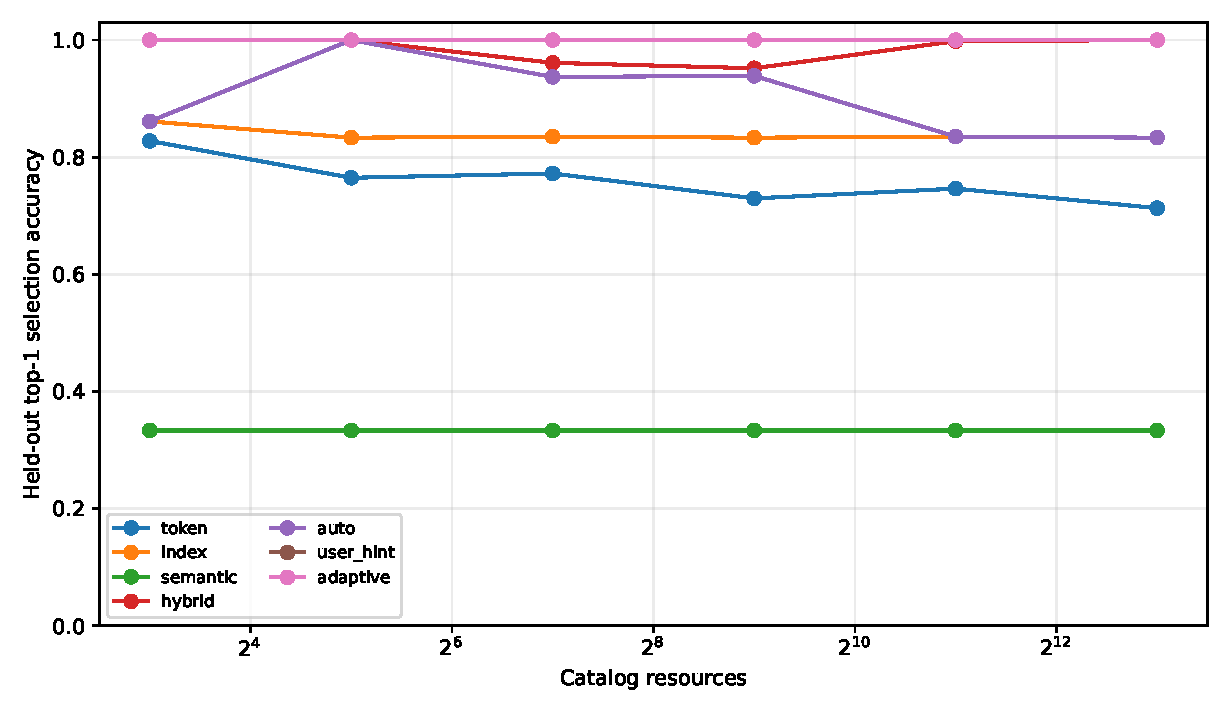
\includegraphics[width=.82\linewidth]{../shared/results/paper6_5_tools/m0_policy_scaling.pdf}
\caption{Positive-request top-1 accuracy as catalog size increases. Ranking
alone does not encode whether confidence permits selection.}
\label{fig:scaling}
\end{figure}

Figure~\ref{fig:scaling} shows that hints and adaptive fallback maintain 1.0
top-1 at every tested size. The result is not uniformly safe at the smallest
size: in the 8-resource condition each policy attains 1.0 positive top-1, but
hinted and adaptive routing each falsely select the ambiguous held-out case in
all five seeds. Their overall outcome accuracy is .974 and safe-nonaction rate
is .5. From 32 resources onward, both negative cases are handled correctly in
all seeds. This inversion is a calibration artifact of the controlled score
distribution and cautions against treating larger catalogs as automatically
harder along every axis.

\subsection{No fixed channel is the oracle everywhere}
At 8,192 resources, the least-cost correct oracle chooses explicit lookup for
16.7\% of positive requests, indexed lookup for 66.7\%, and semantic lookup for
16.7\%. Neither token nor hybrid is ever the least-cost correct choice. User
hints have zero quality regret and 0.083 cost-regret units, compared with zero
quality regret and 0.5 cost regret for adaptive fallback. This supports a
narrow claim: when callers know the reference form, passing that information
avoids discovery work; adaptive escalation remains useful when they do not.

\begin{figure}[H]
\centering
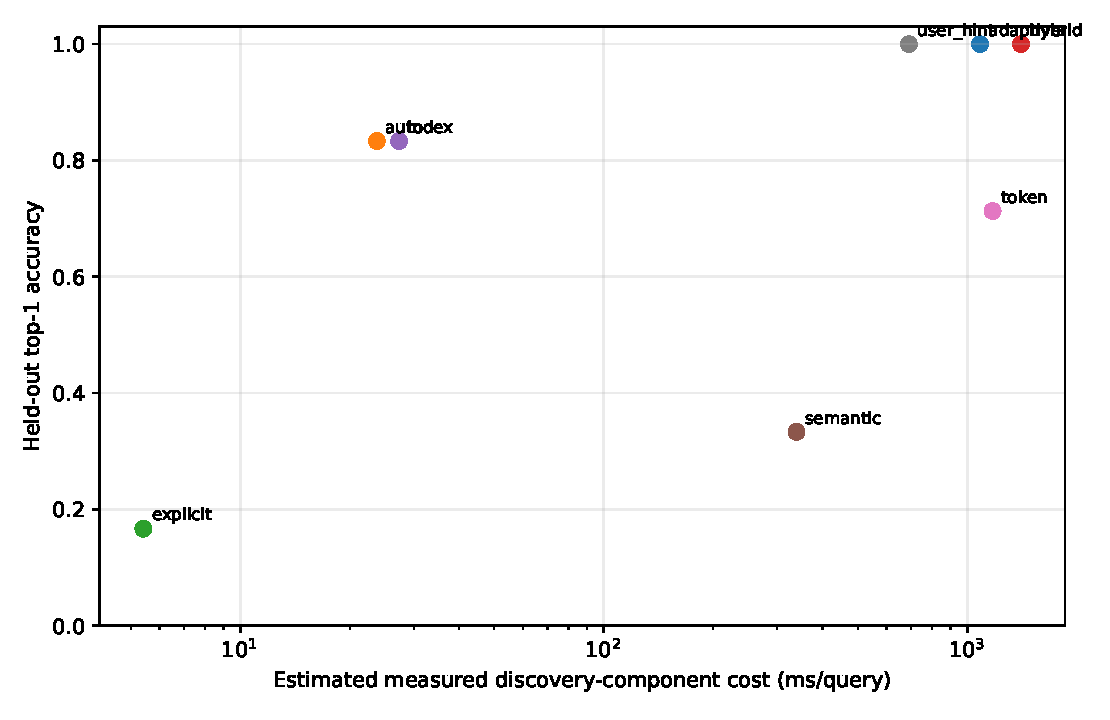
\includegraphics[width=.76\linewidth]{../shared/results/paper6_5_tools/m0_policy_frontier.pdf}
\caption{Largest-catalog ranking quality versus measured discovery-component
cost. The log axis is needed because explicit and exhaustive hybrid paths
differ by more than two orders of magnitude.}
\label{fig:frontier}
\end{figure}

\subsection{Logical catalog size is not active materialization}
Every generated definition contains 18 accounting tokens. The largest catalog
therefore contains 147,456 logical definition tokens, whereas resolving one
resource requests 18 tokens, or 0.0122\% of the catalog. Figure
\ref{fig:context} makes that distinction visible. The number is an accounting
upper bound on selected source text; M0 does not encode definitions into native
K/V and therefore does not establish attention-memory or latency savings.

\begin{figure}[H]
\centering
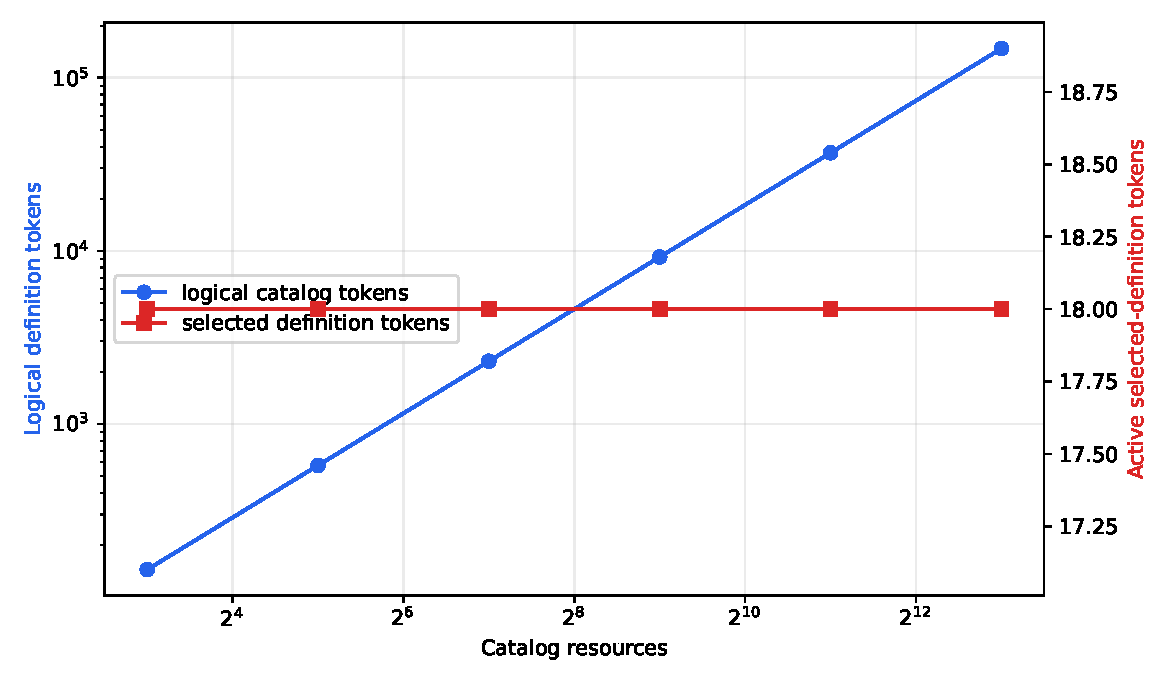
\includegraphics[width=.78\linewidth]{../shared/results/paper6_5_tools/m0_context_scaling.pdf}
\caption{Logical catalog definitions grow with catalog size while the one-item
selected-definition accounting remains at 18 tokens. The axes intentionally
separate logical storage from active materialization.}
\label{fig:context}
\end{figure}

\subsection{Persistent indexing helps, but is not yet production-ready}
At 8,192 resources, index construction takes 1.727 s, a full rebuild after a
one-percent version mutation takes 1.753 s, and the estimated Python index
payload is 5.27 MiB. Warm indexed lookup takes 27.4 ms and scores 966 candidates
on average (11.8\% of the catalog). By comparison, exhaustive semantic, token,
and hybrid controls take 339, 1,174, and 1,405 ms. The index build amortizes to
44.6 ms/query after 100 uses and 29.1 ms after 1,000 uses.

\begin{figure}[H]
\centering
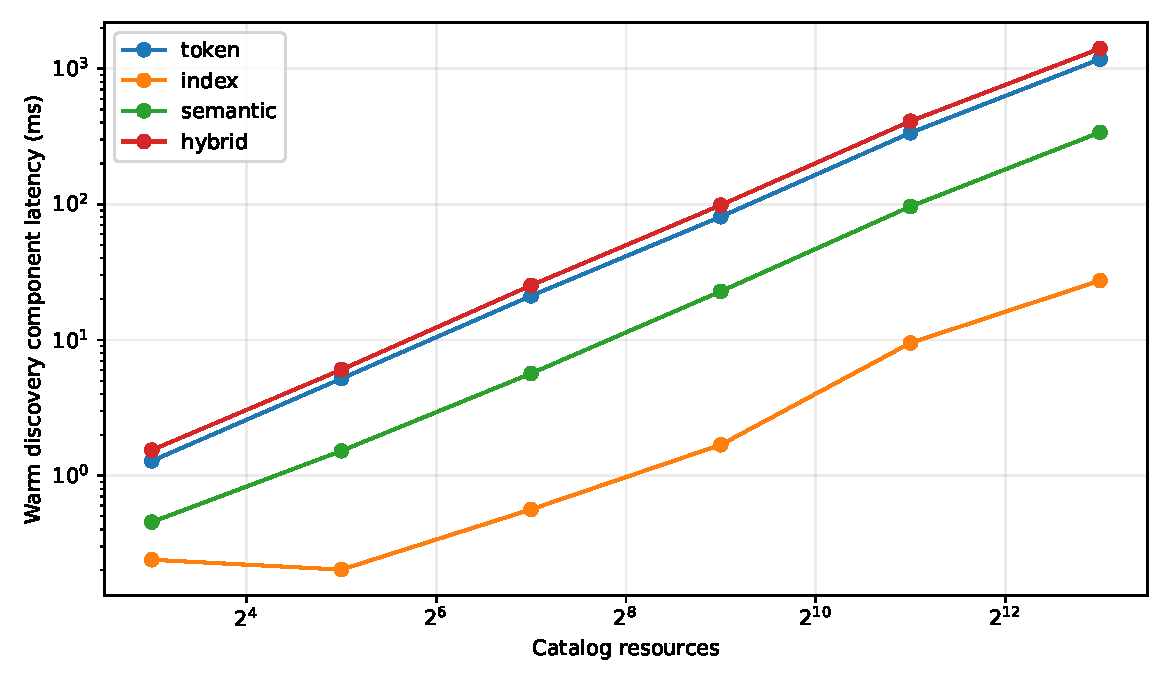
\includegraphics[width=.75\linewidth]{../shared/results/paper6_5_tools/m0_index_latency.pdf}
\caption{Warm CPU Python component latency. Exhaustive channels scale poorly;
the indexed path narrows candidates but still touches about 11.8\% at 8K.}
\label{fig:index}
\end{figure}

These numbers establish an optimization target rather than a speed claim.
Production token postings should avoid Python object traversal, semantic search
should use an approximate vector index, unions should be deduplicated before
scoring, and mutation should update affected postings rather than rebuild the
entire immutable index. Cold/warm serving measurements must also include
tokenization and downstream native-K/V work.

\section{What the M0 Gate Establishes}
The mechanism satisfies four narrow requirements. First, typed resources can be
resolved without exposing the full catalog to a language model. Second,
different reference forms favor different channels. Third, request hints can
match adaptive quality with fewer stages. Fourth, action-aware calibration can
distinguish a correct ranking from a decision safe enough to use.

M0 alone does \emph{not} satisfy the paper's broader context gate. Its 18-token
active count is not a measured model working set. There is no model-side
argument generation, observation-conditioned continuation, persistent-history
recall, skill composition, or subagent inheritance. Its negative controls are
small and its semantic control is idealized. We therefore treat M0 as resolver
evidence rather than evidence that PRA improves agents.

\section{M1: A Causal Toy-Model Gate}
\subsection{Protocol separates discovery, generation, and execution}
The synthetic language gives each tool an opaque identity and a compact
definition. Semantics appear only in that definition. A held-out query states
an action, object, family, and raw argument, but contains neither the resource
identity nor one of four formatting schemas. The host first discovers a stable
URI and binds it to a temporary slot such as \texttt{@0}. The model must emit
\texttt{slot|schema|argument}; the host resolves the slot and accepts the call
only when the selected URI, schema, and formatted argument are all exact. A
deterministic observation is then supplied and the model must continue with the
expected answer. No external side effect is performed.

This boundary matters. Discovery quality is measured by stable URI identity.
The model is responsible for schema-conditioned call construction. The host is
responsible for binding and validation. A correct retrieval cannot receive
end-to-end credit for an incorrect call, and a memorized call string cannot
receive selection credit for an incorrect resource.

\subsection{Model, training, and causal conditions}
The character-level decoder has 506,400 parameters, four layers, hidden width
96, feed-forward width 384, RoPE, and PRA native-K/V at layers 1 and 3. Each of
five seeds trains for 3,000 steps with a mixture of native-memory examples
(50\%), directly presented selected definitions (30\%), and eager eight-item
catalogs (20\%). Loss is applied only to the call and post-observation
continuation. Evaluation uses eight examples per seed at catalog sizes 8, 32,
and 128.

We compare oracle memory, idealized semantically discovered memory, shuffled
memory, disabled memory, the selected definition directly in the native prompt,
and the eager catalog. All conditions share model weights. Shuffling preserves
memory presence and size but selects the wrong definition; disabling removes
memory. Eager conditions that exceed the 512-token native window are recorded
as context overflow and are not truncated into an easier task.

\subsection{Selected native K/V is used causally}
Table~\ref{tab:m1-e2e} reports the strict end-to-end metric: correct resource,
exact call, and exact continuation. Discovered memory matches oracle memory at
all three sizes. Shuffled and disabled conditions obtain zero, so performance
cannot be explained by the query alone or by generic memory activation.

\begin{table}[H]
\centering
\small
\caption{M1 end-to-end success, averaged over five seeds and eight held-out
examples per seed. A dash denotes native-window overflow rather than failure.}
\label{tab:m1-e2e}
\begin{tabular}{lrrrrrr}
\toprule
Catalog & Discovered & Oracle & Direct & Shuffled & Disabled & Eager \\
\midrule
8 & \PaperSixFiveMOneDiscoveredEight & \PaperSixFiveMOneOracleEight & \PaperSixFiveMOneDirectEight & \PaperSixFiveMOneShuffledEight & \PaperSixFiveMOneDisabledEight & \PaperSixFiveMOneEagerEight \\
32 & \PaperSixFiveMOneDiscoveredThirtyTwo & \PaperSixFiveMOneOracleThirtyTwo & \PaperSixFiveMOneDirectThirtyTwo & \PaperSixFiveMOneShuffledThirtyTwo & \PaperSixFiveMOneDisabledThirtyTwo & -- \\
128 & \PaperSixFiveMOneDiscoveredOneTwentyEight & \PaperSixFiveMOneOracleOneTwentyEight & \PaperSixFiveMOneDirectOneTwentyEight & \PaperSixFiveMOneShuffledOneTwentyEight & \PaperSixFiveMOneDisabledOneTwentyEight & -- \\
\bottomrule
\end{tabular}
\end{table}

\begin{figure}[H]
\centering
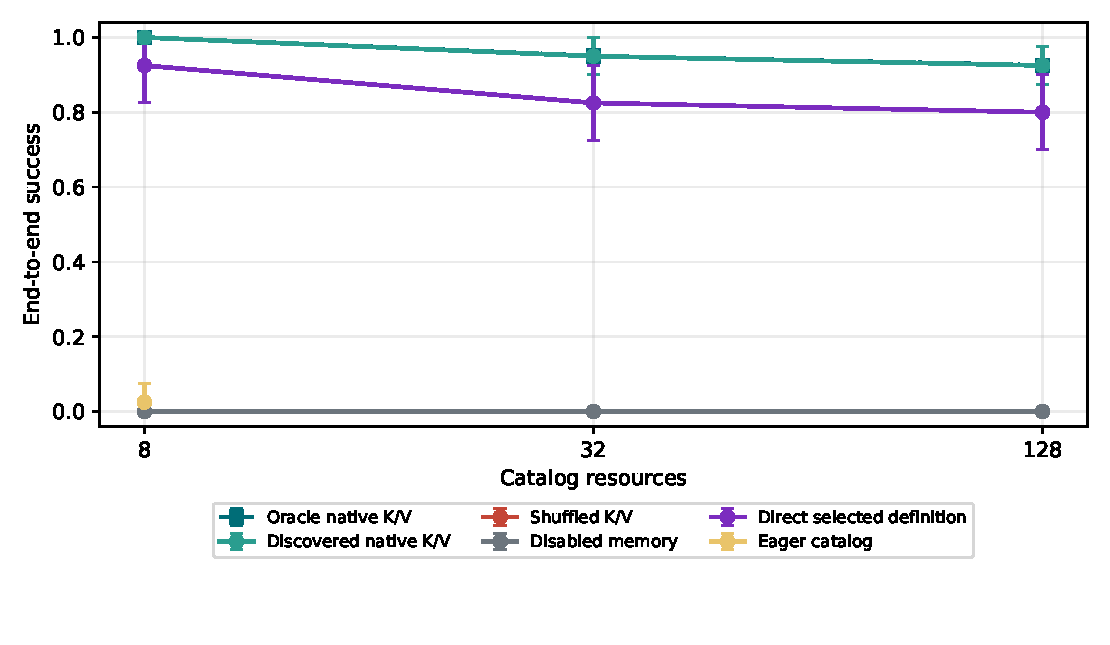
\includegraphics[width=.88\linewidth]{../shared/results/paper6_5_tools/m1/figures/m1_end_to_end_scaling.pdf}
\caption{M1 end-to-end success. Oracle and discovered curves overlap; shuffled
and disabled controls remain at zero. Eager evaluation is defined only where
the complete catalog fits.}
\label{fig:m1-e2e}
\end{figure}

Every seed favors oracle memory over shuffled and disabled memory at every
catalog size. With five paired seeds, however, the minimum attainable exact
two-sided sign-flip value is $p=.0625$. Oracle and discovered memory have zero
paired difference. Direct presentation is lower by .075 at size 8 and .125 at
sizes 32 and 128, but those paired differences are not statistically decisive.
We report the direction without claiming that PRA presentation is intrinsically
better than direct presentation.

\subsection{Logical growth is separated from active K/V}
Figure~\ref{fig:m1-context} measures the neural working set that M0 could only
account for. Logical catalog text grows with catalog size and crosses the
native window before size 32. The selected native-K/V payload remains near one
definition per PRA layer. Direct selected-definition prompts also remain
bounded, making them the relevant non-PRA control. This is evidence of bounded
active materialization in the toy implementation, not a production memory or
latency claim.

\begin{figure}[H]
\centering
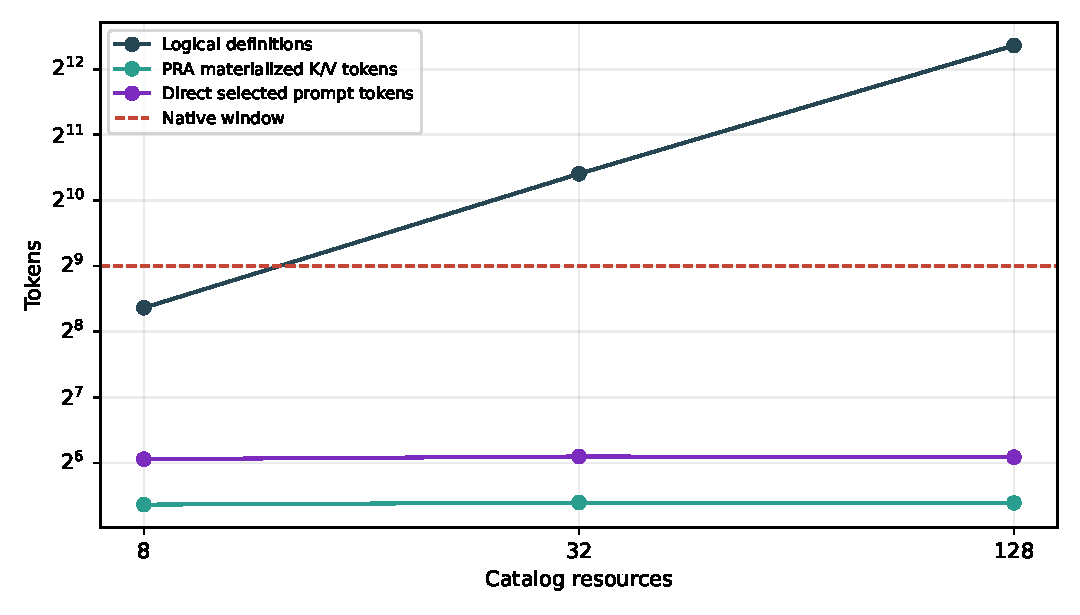
\includegraphics[width=.86\linewidth]{../shared/results/paper6_5_tools/m1/figures/m1_context_accounting.pdf}
\caption{M1 logical catalog text, materialized native K/V per PRA layer, direct
selected prompt length, and the 512-token native window. Logical storage and
attention-visible working memory are distinct quantities.}
\label{fig:m1-context}
\end{figure}

The causal result remains narrow. The semantic discoverer is an idealized
control, not a learned production index. The grammar is synthetic, the executor
is pure and deterministic, and the decoder is trained specifically for this
task. The experiment establishes that the selected native K/V carries necessary
information through call construction and observation-conditioned continuation;
it does not establish general tool use.

\section{M2--M4: From Selection to Typed Execution}
\subsection{Frozen pretrained bridge}
M2 freezes Qwen3-0.6B at revision
\texttt{c1899de289a04d12100db370d81485cdf75e47ca}. Four realistic single-tool
tasks cross five deterministic prompt presentations. The model receives
OpenAI-compatible function schemas and must emit one parseable
\texttt{<tool\_call>} with the exact function and arguments. Conditions expose
the selected tool, the identical oracle tool, a same-family shuffled tool, an
irrelevant tool, no tools, or all 18 catalog tools. The five presentations vary
instruction wording and eager order; they are not independent model-training
seeds.

Selected and oracle disclosure both obtain \PaperSixFiveMTwoSelected\ strict
success (20/20). Shuffled, irrelevant, and empty conditions obtain 0/20. Eager
disclosure obtains \PaperSixFiveMTwoEager\ (17/20). Thus the selected schema
causes the output and a small model can use it without task-specific training;
the eager catalog is not an oracle and already introduces interference.

\subsection{Safe execution and typed observations}
M3 inserts a host boundary after generation. The parser treats model JSON as
untrusted. The executor checks that the function was disclosed, the stable URI
was authorized, required arguments and types match the schema, and write or
destructive authority was granted separately. Only registered pure in-memory
handlers can run. A result becomes
\begin{verbatim}
!!ref:observation:<namespace>:<call-id>:v1!!
\end{verbatim}
with producer URI, result schema, call identity, tenant, and provenance. Tool
outputs are therefore retrievable resources rather than irreversible transcript
text. All 20 selected calls execute and create typed observations. In 17/20
continuations (\PaperSixFiveMThreeGrounded), the model includes every returned
value. The remaining three are consumption failures, despite correct execution.

\subsection{Reactive multi-tool composition}
M4 uses three held-out workflows of length three, four, and five. Reactive JIT
shows only the next discovered schema after each typed result; eager-required
shows the complete evaluator-required set at every step; no-refresh leaves only
the initial tool visible. The same model and prompt presentations are used.
Strict task success requires every expected identity, exact arguments, accepted
execution, and typed observation in order.

\begin{figure}[H]
\centering
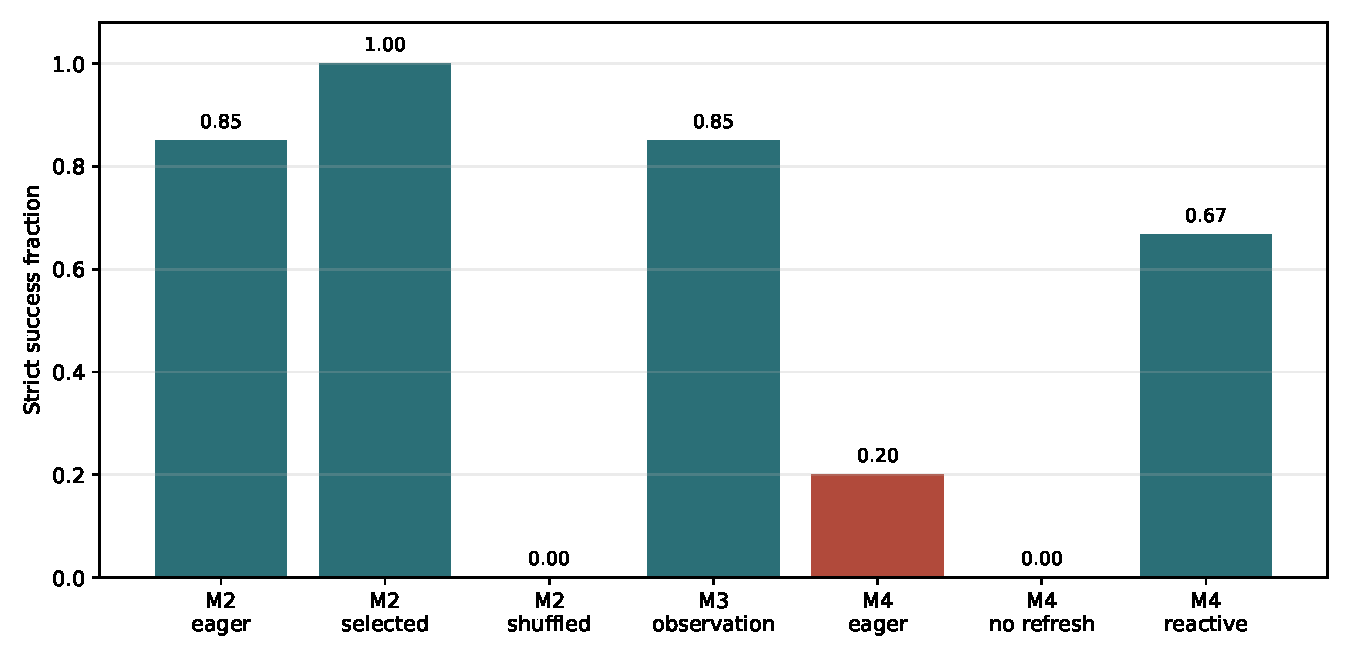
\includegraphics[width=.94\linewidth]{../shared/results/paper6_5_tools/m2_m6_summary/m2_m4_gate_summary.pdf}
\caption{M2--M4 strict gates. Selected definitions cause exact pretrained calls;
typed execution is reliable, while observation consumption remains imperfect.
Reactive disclosure substantially outperforms both a static required set and a
no-refresh control on the small workflow cohort.}
\label{fig:m2-m4}
\end{figure}

Reactive JIT completes \PaperSixFiveMFourReactive\ (10/15), eager-required
\PaperSixFiveMFourEager\ (3/15), and no-refresh 0/15. The three- and four-step
families account for the reactive successes; the five-step cross-domain
repository workflow fails after its first result in every presentation. M4 is
therefore a positive reactive-composition gate, not general long-horizon agent
competence.

\section{M5: Speculative Capability Disclosure}
M5 asks whether exposing a useful capability neighborhood before the first call
improves planning relative to direct Top-1 or reactive retrieval. The 18-node
graph has 171 typed edges. We compare all-tools eager (P0), direct Top-1 and
Top-$K$ (P1--P2), family/category, tag/keyword, and schema expansion (P3--P5),
their bounded union (P6), reactive JIT (P7), horizon-matched speculative
disclosure (P8), and the exact required set (P9). Labels distinguish required,
useful, related-but-unnecessary, irrelevant, and unsafe tools.

\begin{table}[H]
\centering
\small
\caption{M5 capability-set and execution results over three workflows. Recall
and initial tool counts are averaged across tasks. Model success has 15 trials
for P1, P6--P9; a dash denotes a set-only policy.}
\label{tab:m5}
\begin{tabular}{lrrrr}
\toprule
Policy & Required recall & Initial tools & Unsafe & Model success \\
\midrule
P0 all eager & 1.000 & 18.00 & 1.00 & -- \\
P1 direct Top-1 & .261 & 1.00 & 0 & .000 \\
P2 direct Top-$K$ & .822 & 4.00 & 0 & -- \\
P5 schema graph & .628 & 3.67 & 0 & -- \\
P6 combined graph & \PaperSixFiveMFiveCombinedRecall & 6.67 & 0 & \PaperSixFiveMFiveCombinedSuccess \\
P7 reactive JIT & .261 & 1.00 & 0 & .667 \\
P8 speculative matched & .628 & 3.67 & 0 & .000 \\
P9 oracle capabilities & 1.000 & 4.00 & 0 & .200 \\
\bottomrule
\end{tabular}
\end{table}

\begin{figure}[H]
\centering
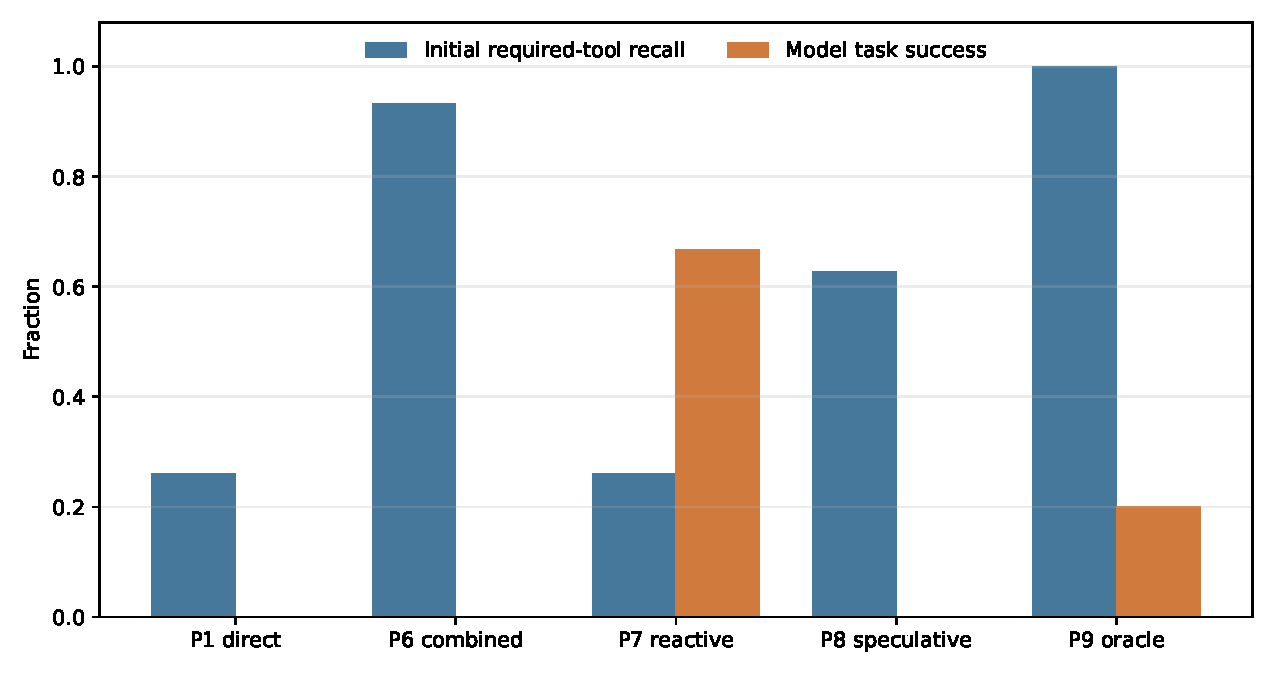
\includegraphics[width=.90\linewidth]{../shared/results/paper6_5_tools/m2_m6_summary/m5_recall_vs_execution.pdf}
\caption{Initial required-tool recall is not task success. The combined graph
recovers most required capabilities without unsafe exposure, yet the frozen
model does not execute successfully from the larger static set.}
\label{fig:m5}
\end{figure}

The M5 stop/go gate is negative. P6 fully covers two workflows and reaches
.933 mean required recall, but static P6 and P8 disclosure obtain 0/15 model
success. Even P9 obtains only 3/15, whereas P7 reactive JIT obtains 10/15. The
experiment does not support training an adaptive disclosure controller. The
fixed graph remains useful for auditable candidate construction, but a useful
capability set expands the action space; it does not solve action sequencing.

\section{M6: Optional PRA-Native Resource Discovery}
Native Q/K is not treated as another ordinary SDK function. In a generic
deployment, the agent and resolver sit outside an opaque model API and cannot
read hidden states, native query vectors, key vectors, or PRA cache entries.
M6 therefore defines four explicit arrangements: co-located execution; a
same-host shared-memory index that exports only $z_q=W_q q$; a model-server
resolver endpoint that returns typed URIs and scores; and replicated query
computation requiring the same model, tokenizer, layer, projection, and
position treatment. Only the co-located mechanism is executed here. The SDK
also implements the projected-query payload and identity-only server reply;
raw Q/K is not persisted in artifacts.

At frozen Qwen layer 27, 1,625 tokens from 18 structured definitions are
encoded with explicit name, description, parameter, return, side-effect, and
tag boundaries. Five prompt presentations cover four single-tool and three
multi-tool tasks. Baselines include token and indexed lexical routing, a
signed-hash control, input-embedding means, native mean K, full token QK, and a
lexical/native fusion. The rank-16 and rank-8/eight-centroid projections are
the five Paper-2.8 HotpotQA/QASPER checkpoints applied zero-shot; they receive
no tool supervision.

\begin{table}[H]
\centering
\small
\caption{M6 co-located discovery. Multi-step recall uses a budget equal to the
workflow horizon. Bytes are declared persistent routing-index payloads, not
Python/process overhead or backing native K/V.}
\label{tab:m6}
\begin{tabular}{lrrrr}
\toprule
Mode & Single Top-1 & Multi recall & Successor recall & Index bytes \\
\midrule
Token & .800 & .889 & 1.000 & 13,427 \\
Index & \PaperSixFiveMSixIndexTopOne & .862 & 1.000 & 13,427 \\
Signed hash & .800 & .670 & .906 & 9,216 \\
Input-embedding mean & .650 & .619 & .572 & 36,864 \\
Lexical + rank-16 & .800 & .690 & .689 & 65,427 \\
Native mean K & \PaperSixFiveMSixNativeMeanTopOne & .439 & .611 & 36,864 \\
Native token QK & .000 & .439 & .611 & 3,328,000 \\
Paper-2.8 rank-16 & .000 & \PaperSixFiveMSixRankSixteenRecall & .167 & 52,000 \\
Paper-2.8 rank-8/8-centroid & .000 & .372 & .167 & 2,304 \\
\bottomrule
\end{tabular}
\end{table}

\begin{figure}[H]
\centering
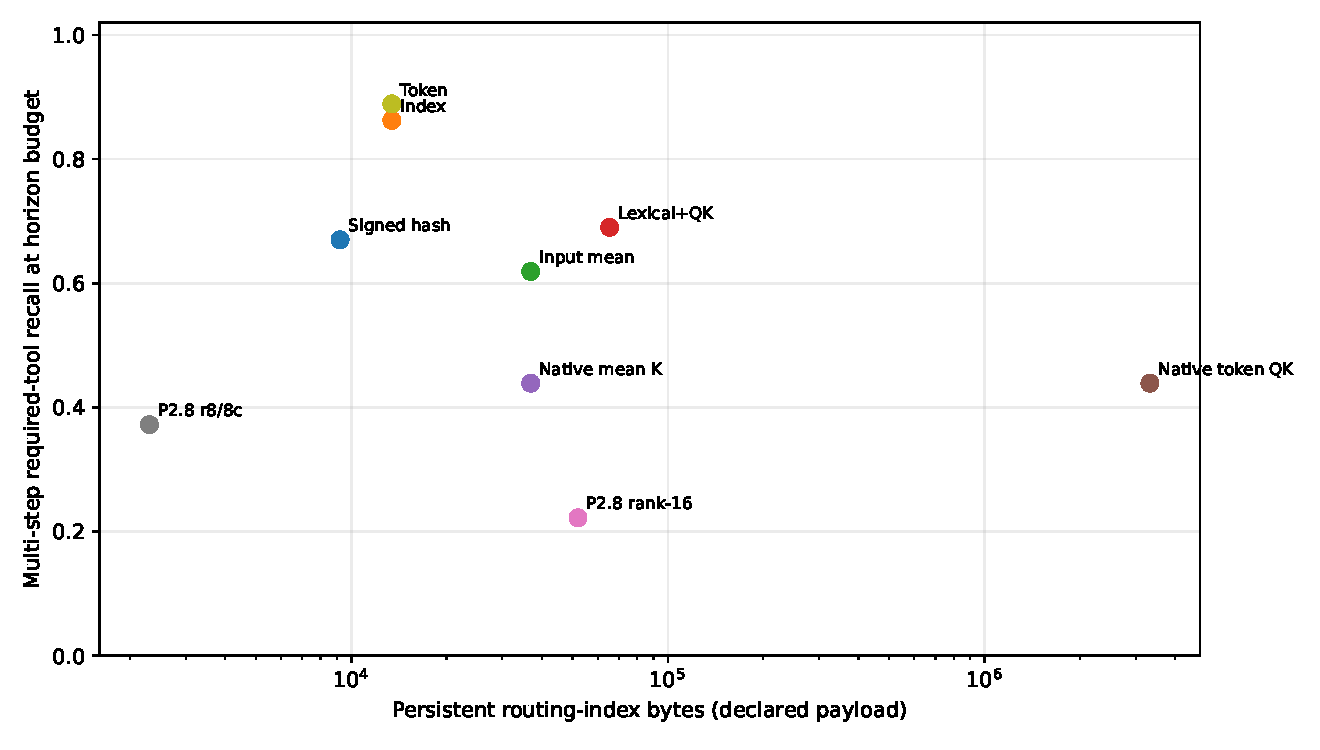
\includegraphics[width=.76\linewidth]{../shared/results/paper6_5_tools/m2_m6_summary/m6_quality_cost_frontier.pdf}
\caption{M6 multi-step retrieval quality against routing-index payload. The
compact transferred projection is inexpensive, but lexical channels dominate
quality on this catalog. Full native-token scoring is both worse and larger.}
\label{fig:m6}
\end{figure}

M6 also stops negatively. Native query/key state does not improve this tool
catalog, and the QA-trained low-rank map does not transfer to capability
language. The lexical/native fusion is below either lexical channel alone.
Consequently the supported generic architecture remains external
explicit/token/index discovery. Model-server native routing is an optional
research interface whose tighter coupling is not justified by these results.

\section{M6.5: External Semantic-Hard Discovery}
\subsection{Frozen benchmark and split discipline}
M6 answers a canonical-language question; it does not show that lexical search
is sufficient for sloppy intent. We therefore freeze 306 single-tool requests
over the same 18-tool catalog. Each identity has one held-out test and one
validation realization in H0 (canonical), H1 (synonym), H2 (colloquial), H3
(implicit goal), H4 (bounded context plus shorthand), and H5 (Portuguese,
Spanish, or French against English tool definitions). Eighteen additional
audit rows cover the catalog. Validation and test contain 144 identities each;
the complete query fingerprint is
\texttt{e348334ad2362f284a217f1f852f175917a17540dd403f79953d7d2a7ebd7adb}.
For H2 and later, tests reject exact tool names and aliases. H4 gives every
channel the same context. No test wording selects an encoder, representation,
fusion weight, or confidence threshold.

This is a controlled, project-authored fixture rather than a naturally sampled
user corpus. Its multilingual mappings and tool tags share the benchmark's
typed concept inventory. Their accuracy measures the value of registration-time
semantic metadata under those declared assumptions, not open-domain translation
or multilingual generalization. The benchmark evaluates discovery only; the
multi-step planning and execution boundaries remain those measured in M4--M5.

\subsection{External policies}
The concept map resolves domain-bounded operation/object phrases and retains
language, source, and weight for every expansion. Tool registration emits four
representations: description; name plus description; a deterministic card with
purpose, operation, object, input/output types, and side effect; and three
separate vectors for those fields. Three compact encoders are selected on
validation only: all-MiniLM-L6-v2, BGE-small-en-v1.5, and multilingual
MiniLM-L12-v2, all pinned by revision. Validation selects BGE with description
cards and context-plus-query for English, and multilingual MiniLM with
structured cards and query-only encoding for H5. Tool vectors are persisted;
third-party weights are not copied into the repository.

The policy ladder compares token overlap (P0), BM25 (P1), typed dictionary
expansion (P2), registration-time tags (P3), their lexical combinations,
English and multilingual embeddings, a validation-frozen hybrid, and an
identity oracle. A staged P10 resolver tries lexical, dictionary/tags, and the
embedding hybrid before asking. Its four thresholds are fitted on validation.

\begin{table}[H]
\centering
\small
\caption{M6.5 results on \PaperSixFiveSemanticTestQueries{} frozen test
requests. Latency is the median measured end-to-end resolver time for this
18-candidate Python implementation; embedding registration is amortized.}
\label{tab:m65}
\begin{tabular}{lrrrr}
\toprule
Policy & Top-1 & MRR & Recall@3 & Median ms \\
\midrule
Token & .257 & .398 & .403 & 8.6 \\
BM25 & \PaperSixFiveSemanticBMTopOne & .485 & .514 & 8.6 \\
Typed dictionary & .729 & .812 & .868 & 8.6 \\
Registration tags & \PaperSixFiveSemanticTagsTopOne & .823 & .875 & 8.6 \\
English embedding & .563 & .682 & .750 & 12.3 \\
Multilingual embedding & .556 & .690 & .785 & 10.8 \\
Dictionary/embedding hybrid & \PaperSixFiveSemanticHybridTopOne & .809 & \PaperSixFiveSemanticHybridRecallThree & 12.3 \\
Identity oracle & 1.000 & 1.000 & 1.000 & 8.6 \\
\bottomrule
\end{tabular}
\end{table}

Tags improve Top-1 over BM25 by \PaperSixFiveSemanticTagGain{} (paired
identity bootstrap 95\% interval
[\PaperSixFiveSemanticTagGainLow{}, \PaperSixFiveSemanticTagGainHigh{}]; exact
discordance $p<10^{-10}$). The gain is not uniform. English BGE is strongest
on H3 implicit goals (.722), tags on H4 context (.556), and curated tags are
perfect on H5 because all three languages are represented in the frozen
concept inventory. The hybrid improves H2 to .667 and H5 to .963 but does not
dominate each specialized channel. This is why the deployment policy is a
calibrated ladder, not a claim that one embedding replaces lexical metadata.

\begin{figure}[H]
\centering
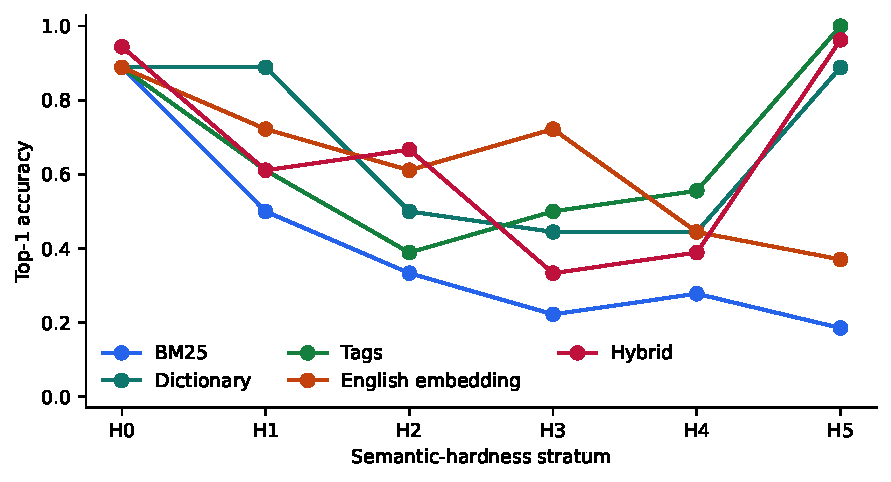
\includegraphics[width=.92\linewidth]{../shared/results/paper6_5_tools/semantic_summary/semantic_quality_by_hardness.pdf}
\caption{External discovery by hardness. Lexical quality declines as canonical
wording disappears; typed metadata and embeddings recover different strata.}
\label{fig:m65-hardness}
\end{figure}

\begin{figure}[H]
\centering
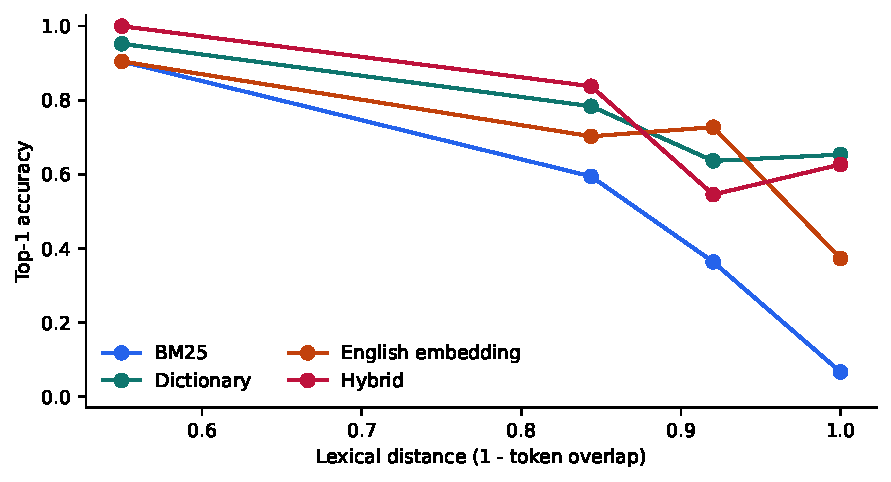
\includegraphics[width=.92\linewidth]{../shared/results/paper6_5_tools/semantic_summary/semantic_quality_vs_lexical_distance.pdf}
\caption{Required quality-versus-distance analysis. Bins contain 21, 37, 11,
and 75 test identities from lower to higher lexical distance. Dictionary and
hybrid channels retain substantial accuracy when token overlap is zero.}
\label{fig:m65-distance}
\end{figure}

\subsection{Selective action and deployment cost}
On test, staged P10 selects 86 of 144 requests and asks on 58: coverage is
\PaperSixFiveSemanticCoverage{}, selective accuracy is
\PaperSixFiveSemanticSelectiveAccuracy{}, actionable accuracy is .542, and the
false-action rate is \PaperSixFiveSemanticFalseAction{}. No selected top tool
is in the row's unsafe set. Its Brier score is \PaperSixFiveSemanticBrier{} and
10-bin ECE is \PaperSixFiveSemanticECE{}. These held-out numbers are weaker than
validation (.949 selective accuracy), which is a reason to retain ASK rather
than lower thresholds after seeing test outcomes.

The 384-dimensional persistent tool vectors occupy 27.6 kB. The selected BGE
encoder has 133.4 MB of parameters, loads into the process in 3.75 s, and encodes the full
306-query cohort in 1.13 s on the recorded CUDA host; its median per-query
resolver path is 12.3 ms versus 8.6 ms for dictionary/tags. The multilingual
encoder is larger (470.6 MB) and is not selected for the generic fusion.

\begin{figure}[H]
\centering
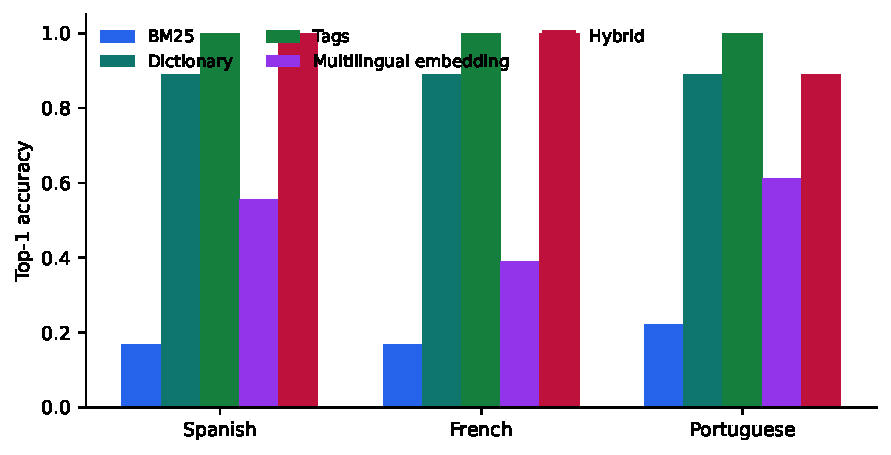
\includegraphics[width=.88\linewidth]{../shared/results/paper6_5_tools/semantic_summary/semantic_multilingual_quality.pdf}
\caption{H5 retrieval against English tool definitions. The curated dictionary
and tag channels encode the three tested languages by construction; the
multilingual encoder is an independent model-backed control.}
\label{fig:m65-language}
\end{figure}

\begin{figure}[H]
\centering
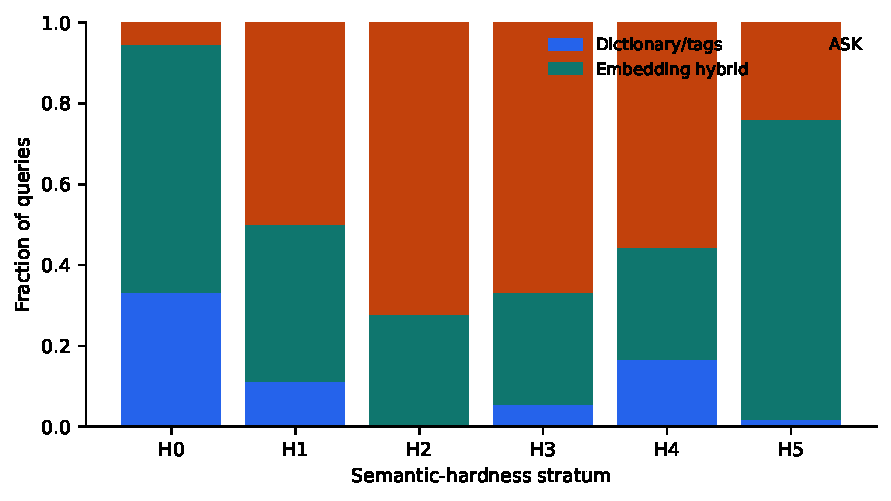
\includegraphics[width=.88\linewidth]{../shared/results/paper6_5_tools/semantic_summary/semantic_staged_escalation.pdf}
\caption{Validation-calibrated P10 stage outcomes on test. More semantic-hard
rows reach the hybrid or ASK stages instead of forcing a low-confidence call.}
\label{fig:m65-stages}
\end{figure}

\section{M7: Native Geometry on the Frozen Hard Set}
M7 reuses all \PaperSixFiveSemanticTestQueries{} test identities without
changing wording, tool cards, or external policies. Frozen Qwen3-0.6B layer-27
pre-RoPE state supplies native mean K and full token QK. The Paper-2.8 rank-16
ensemble and rank-8/eight-centroid ensemble are transferred from five
HotpotQA/QASPER checkpoints without tool supervision. Query encoding is charged
online; raw native state is not persisted.

\begin{table}[H]
\centering
\small
\caption{M7 matched semantic-hard comparison. Model bytes include the frozen
Qwen required to reproduce native queries; index bytes exclude backing model
weights. The rank-8 timing includes the current per-query centroid construction
and is not a production index latency.}
\label{tab:m7}
\begin{tabular}{lrrrr}
\toprule
Mode & Top-1 & MRR & Recall@3 & Median ms \\
\midrule
BM25 & .347 & .485 & .514 & 8.6 \\
Tags & .743 & .823 & .875 & 8.6 \\
English embedding & .563 & .682 & .750 & 12.3 \\
External hybrid & .729 & .809 & .875 & 12.3 \\
Native mean K & \PaperSixFiveMSevenMeanTopOne & .233 & .313 & 116.7 \\
Native token QK & \PaperSixFiveMSevenTokenTopOne & .220 & .181 & 115.9 \\
Paper-2.8 rank-16 & \PaperSixFiveMSevenRankSixteenTopOne & .194 & .167 & 122.9 \\
Paper-2.8 rank-8/8-centroid & \PaperSixFiveMSevenRankEightTopOne & .190 & .167 & 1,658.4 \\
\bottomrule
\end{tabular}
\end{table}

The native Top-1 range, .049--.063, contains the uniform catalog chance rate
$1/18=.056$. Tags exceed native mean K by .688 (paired bootstrap 95\% interval
[.604,.764]) and full token QK by .681 ([.597,.764]). Thus the harder wording
does not reveal a frozen native advantage hidden by M6's canonical queries.
This result is narrower than ``native Q/K cannot encode tool intent'': it says
that one frozen layer, two direct reducers, and QA-trained low-rank projections
do not expose it zero-shot for this catalog.

Tool-specific native training does not open. External accuracy leaves oracle
headroom, but none of the four frozen native diagnostics supplies the required
positive signal, and reproducing native queries requires a 1.19 GB model plus
co-location or a model-server extension. The next justified experiment would
need tool-supervised evidence independent of this test set, not adaptation to
the 144 held-out requests.

\begin{figure}[H]
\centering
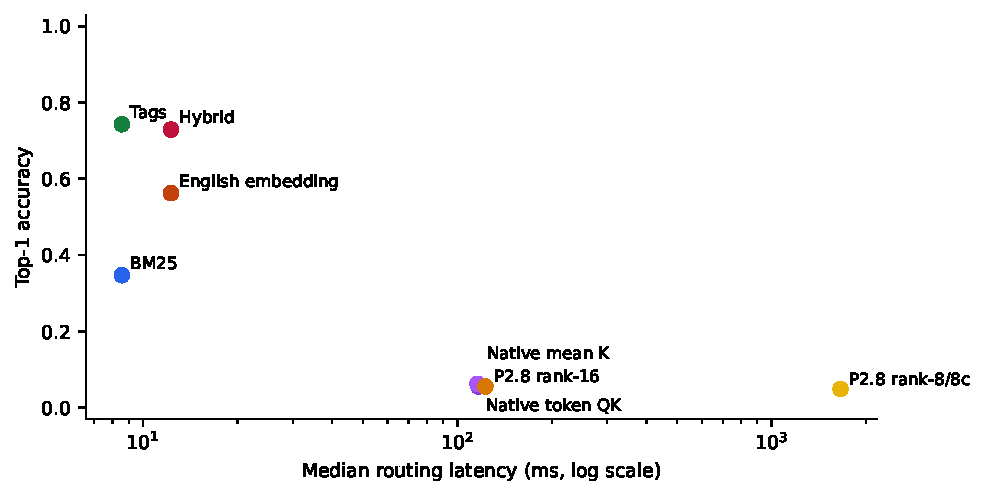
\includegraphics[width=.90\linewidth]{../shared/results/paper6_5_tools/semantic_summary/semantic_quality_latency_frontier.pdf}
\caption{M7 quality--latency frontier on matched queries. External typed
semantics dominates the tested frozen native modes in both quality and online
latency on this small catalog.}
\label{fig:m7-frontier}
\end{figure}

\section{M8: Automatic Tool Records and Record-Aware Materialization}
\subsection{Ordinary callables become typed resources}
M6.5's curated registration metadata raises an adoption question: must every
function author learn a PRA-specific vocabulary? M8 adds
\texttt{tool\_record\_from\_callable}, which inspects but never invokes a Python
callable. It preserves module and qualified name, sync/async status, signature,
parameter kinds and defaults, input and return annotations, and descriptions
parsed from Google, NumPy, or Sphinx-style docstrings. A provider-independent
\texttt{ToolSchema} exports to provider formats only at the boundary. Its type
cache covers primitives, generic containers, optional and union types,
\texttt{Literal}, enumerations, dataclasses, \texttt{TypedDict}, annotated
classes, and Pydantic when installed; no optional dependency is required.

Semantic enrichment remains auditable. Function-name terms, parameter and
return types, docstring terms, canonical operation/object concepts, and
dictionary expansions retain source and deterministic weight. Curated and
automatic tags occupy separate fields. Generic verbs such as \texttt{get} and
\texttt{read} can establish operation type without receiving the same lexical
weight as \texttt{delete} or \texttt{update}. Name-inferred destructive
operations are conservatively hidden from ordinary disclosure, but this hint
does not grant or replace host execution authority.

E1 aligns 18 ordinary annotated callables with the existing rich catalog and
uses the same 144 frozen test requests. Fusion weights are selected only on the
144 validation requests. The automatic hybrid obtains
\PaperSixFiveAutoTopOne{} Top-1 and \PaperSixFiveAutoRecallThree{} Recall@3,
compared with \PaperSixFiveManualTopOne{} Top-1 for the rich manual hybrid.
Thus automatic metadata retains all measured gain over its lexical baseline in
this controlled catalog. This is evidence for a low-annotation registration
path, not evidence that docstrings are always complete or that inferred risk
metadata is authorization.

\begin{figure}[H]
\centering
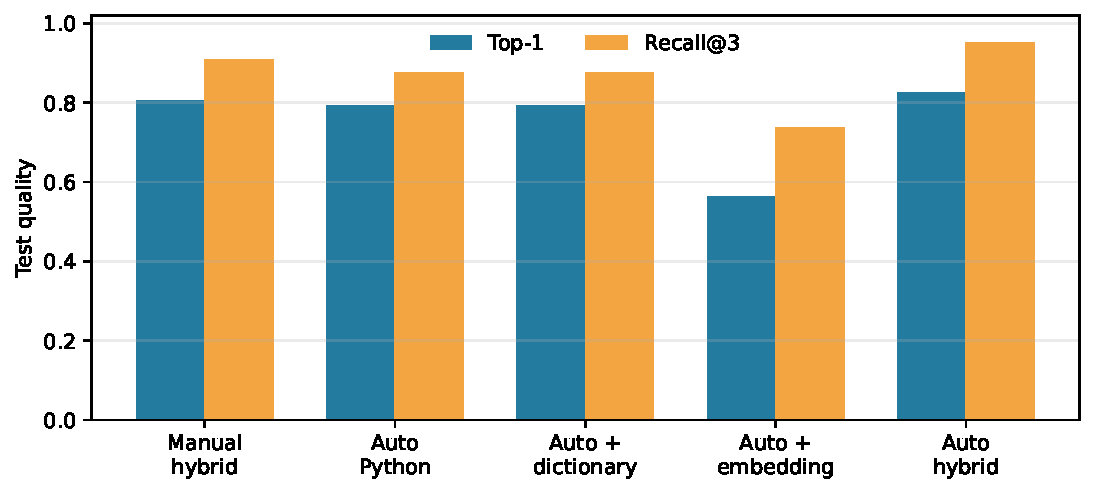
\includegraphics[width=.88\linewidth]{../shared/results/paper6_5_tools/auto_union_records/auto_vs_manual_quality.pdf}
\caption{E1 frozen-test quality. Ordinary signatures and docstrings recover
the rich catalog result after validation-only fusion selection.}
\label{fig:m8-auto}
\end{figure}

\subsection{A zero-configuration ladder identifies the useful signals}
The combined E1 result does not show which automatically derived fields matter.
We therefore freeze one \texttt{ToolRecord} per callable and score every policy
against the same 144 test requests. The record contains only function and
qualified names, module, signature, parameter and return annotations,
descriptions parsed from the docstring, and deterministic fields derived from
them. Every derived term records whether it came from a name, docstring,
parameter, return, type schema, dictionary expansion, inferred operation or
object, automatic tag, or embedding field. No condition receives a per-tool
alias, tag, operation, object, or capability edge.

Table~\ref{tab:m8-auto-ablation} gives the complete ladder. Raw BM25 reaches
\PaperSixFiveAblationRawTopOne{} Top-1. Reweighting automatically extracted
keywords alone raises Recall@3 but lowers Top-1 to
\PaperSixFiveAblationKeywordTopOne{}; extraction is therefore not itself a
semantic resolver. The global, tool-independent synonym dictionary supplies
the largest isolated gain, reaching \PaperSixFiveAblationSynonymTopOne{}
Top-1. Adding inferred concepts and tags by elementwise score maxima does not
improve that ranker in isolation. The selected name-plus-description embedding
is complementary rather than sufficient. A validation-selected mixture of
synonym, automatic-tag, and embedding scores reaches
\PaperSixFiveAblationAutoTopOne{} Top-1 and
\PaperSixFiveAblationAutoRecallThree{} Recall@3, versus
\PaperSixFiveAblationManualTopOne{} and
\PaperSixFiveAblationManualRecallThree{} for manually enriched registration.
The one-row Top-1 difference is not evidence that automatic metadata is
generally superior; it is a parity result on one controlled catalog.

\begin{table}[H]
\centering
\small
\resizebox{\linewidth}{!}{\begin{tabular}{lccccrrr}
\toprule
Policy & Manual & Syn. & Concepts & Embed. & Top-1 & R@3 & R@5 \\
\midrule
A0 Raw BM25 & no & no & no & no & 0.403 & 0.556 & 0.639 \\
A1 Auto keywords & no & no & no & no & 0.306 & 0.597 & 0.681 \\
A2 Keywords + synonyms & no & yes & no & no & 0.750 & 0.882 & 0.910 \\
A3 Inferred concepts & no & yes & yes & no & 0.632 & 0.882 & 0.903 \\
A4 Automatic tags & no & yes & yes & no & 0.618 & 0.875 & 0.903 \\
A5 Compact embedding & no & no & no & yes & 0.556 & 0.764 & 0.840 \\
A6 Automatic hybrid & no & yes & yes & yes & 0.812 & 0.938 & 0.958 \\
A7 raw union ($K=10$) & no & yes & yes & yes & -- & 0.882 & 0.910 \\
Manual-rich ceiling & yes & yes & yes & yes & 0.806 & 0.910 & 0.958 \\
\bottomrule
\end{tabular}
}
\caption{Frozen-test automatic discovery ladder. A7 has no unique Top-1:
R@3 and R@5 evaluate caps three and five, while validation selects raw union at
$K=10$ for its maximum set recall. ``Manual'' denotes per-tool authored
semantic metadata; all A0--A7 fields come from the same callable record.}
\label{tab:m8-auto-ablation}
\end{table}

\begin{figure}[H]
\centering
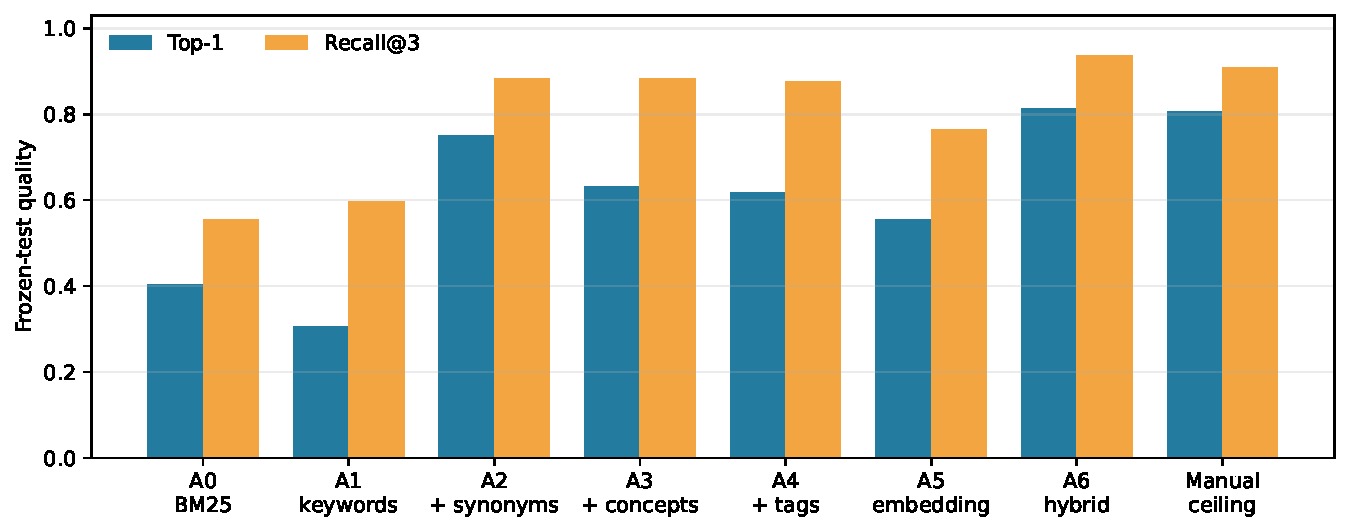
\includegraphics[width=.96\linewidth]{../shared/results/paper6_5_tools/auto_discovery_ablation/auto_discovery_ladder.pdf}
\caption{A0--A6 contribution ladder and the manual-rich control. A5 is an
independent embedding condition rather than an incremental addition to A4;
A6 is the validation-frozen fusion.}
\label{fig:m8-auto-ladder}
\end{figure}

The hardness decomposition in Figure~\ref{fig:m8-auto-hardness} clarifies the
complementarity. BM25 is already strong on direct H0 requests but degrades on
implicit and contextual requests. The generic dictionary dominates the
multilingual H5 fixtures, whereas the English compact embedding is strongest
on H2--H4 paraphrastic and implicit English requests. Their fusion is therefore
more stable than either channel alone. These multilingual rows test the frozen
dictionary coverage, not open-domain translation.

\begin{figure}[H]
\centering
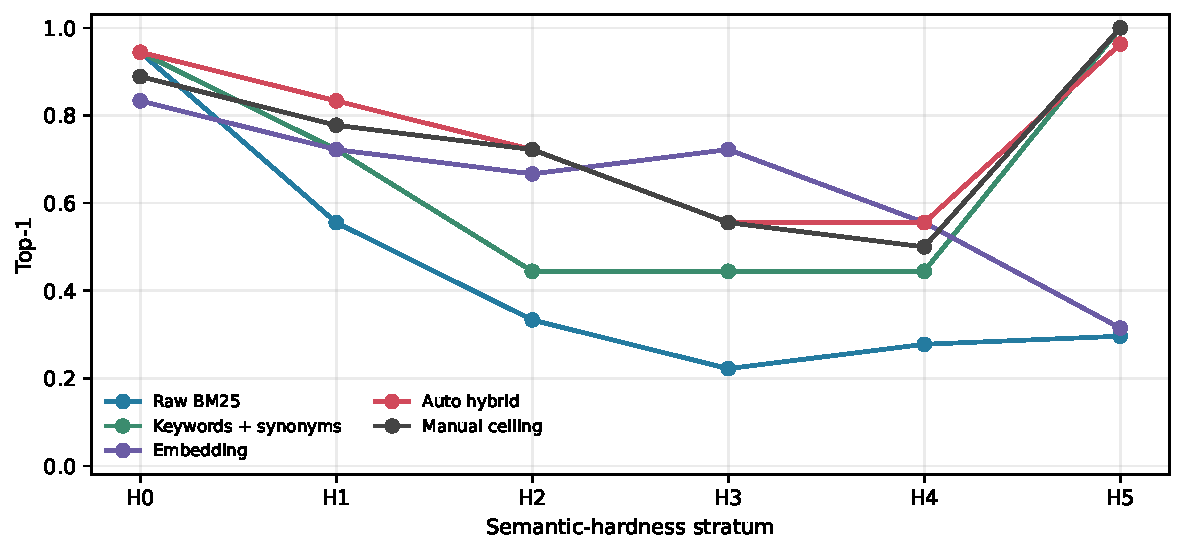
\includegraphics[width=.88\linewidth]{../shared/results/paper6_5_tools/auto_discovery_ablation/auto_discovery_by_hardness.pdf}
\caption{Top-1 by frozen semantic-hardness stratum. The automatic hybrid tracks
the manual ceiling while using different channels for lexical, implicit, and
multilingual requests.}
\label{fig:m8-auto-hardness}
\end{figure}

One-at-a-time source controls locate practical SDK requirements. Removing
docstring terms lowers A1 Recall@3 from .597 to
\PaperSixFiveDocstringRemovalRecallThree{}; type/schema terms add
\PaperSixFiveTypeRecallThreeGain{} Recall@3, although they do not improve A1
Top-1 and do not alter A4. With no docstring, embedding Top-1 falls from .556 to
\PaperSixFiveNoDocEmbeddingTopOne{}. Replacing descriptive names with opaque
identifiers while retaining the docstring and signature yields
\PaperSixFiveOpaqueNameEmbeddingTopOne{}. Thus registration remains useful with
weak names, but documentation quality matters, especially to the embedding
fallback. Figure~\ref{fig:m8-auto-quality} reports these controlled variants;
they do not modify the frozen request text.

\begin{figure}[H]
\centering
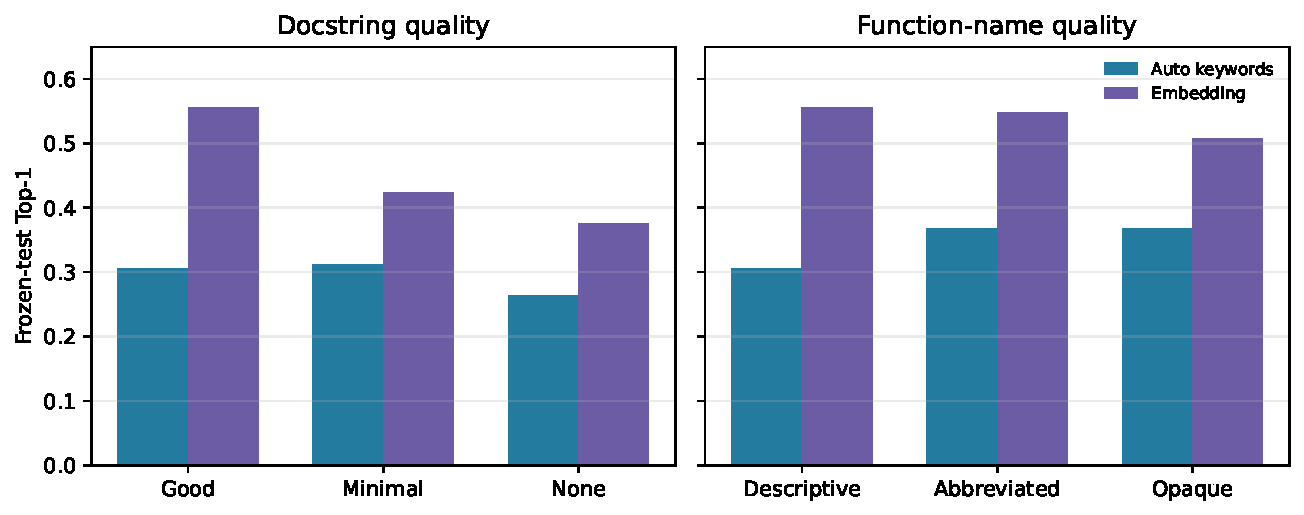
\includegraphics[width=.88\linewidth]{../shared/results/paper6_5_tools/auto_discovery_ablation/auto_callable_quality_sensitivity.pdf}
\caption{Sensitivity to callable documentation and naming. Each intervention
changes only the named source while preserving signatures, target identities,
and requests.}
\label{fig:m8-auto-quality}
\end{figure}

\subsection{Candidate palettes do not reduce to one winner}
The resolver can now return a bounded \texttt{CandidateSet} rather than only a
Top-1 URI. Every candidate retains all channel hits and its admission source;
deduplication uses stable URI. E2 sweeps budgets
$K\in\{1,2,3,4,5,6,8,10\}$ and compares the best single channel, normalized
score fusion, raw union, and a diversity-aware union that admits one unseen
candidate from each enabled channel before filling remaining slots. Metrics
include required/useful recall, useful precision, unsafe exposure, schema
tokens, and provenance diversity.

At $K=4$, fused Top-K reaches \PaperSixFiveFusedKFourRecall{} required-tool
recall versus \PaperSixFiveUnionKFourRecall{} for diversity union. Recall rises
with larger palettes, but useful precision falls and labeled unsafe exposure
increases. The requested default-union gate is therefore negative: candidate
sets are first-class and union remains configurable, while validation-selected
fusion remains the supported semantic palette policy for this cohort.

\begin{figure}[H]
\centering
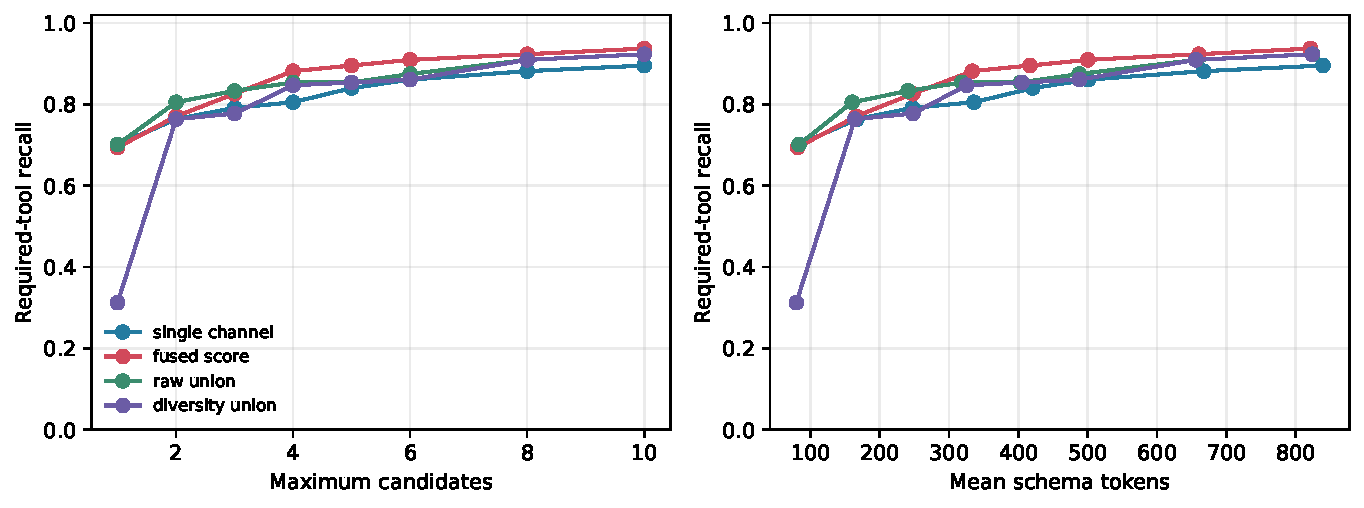
\includegraphics[width=.94\linewidth]{../shared/results/paper6_5_tools/auto_union_records/union_recall_frontier.pdf}
\caption{E2 required-tool recall against candidate count and serialized schema
cost. Diversity preserves channel representation but does not dominate fused
Top-K at matched budgets.}
\label{fig:m8-union}
\end{figure}

The isolated A7 rerun reaches the same decision with five strictly automatic
channels: BM25, extracted keywords, keyword-plus-synonym scores,
automatic-tag/concept scores, and the selected embedding. At $K=4$, fused
Top-K obtains \PaperSixFiveAutoFusedKFourRecall{} required-tool recall, versus
\PaperSixFiveAutoRawUnionKFourRecall{} for raw union and
\PaperSixFiveAutoDiversityKFourRecall{} for diversity union. Validation selects
raw union at $K=10$ if recall is optimized alone; on test it reaches
\PaperSixFiveAutoSelectedUnionRecall{} recall but exposes at least one labeled
unsafe candidate on \PaperSixFiveAutoSelectedUnionUnsafe{} of requests and
serializes 811 mean schema tokens. Channel complementarity is real but sparse:
8 of 144 targets are recovered only by the embedding, 3 only by an automatic
lexical/concept channel, 129 by multiple channels, and 4 by none at per-channel
$K=3$. Larger set size, rather than broad unique recovery, explains most of the
raw-union frontier.

The preregistered automatic-union JIT gate therefore remains closed. No new
generative run is performed: on validation, neither union variant materially
exceeds matched-budget fusion while holding unsafe exposure within one
percentage point. This is an intentional stopped experiment, not missing data.
Candidate provenance and union remain exposed by the SDK for diagnostics and
future cohorts, but validation-frozen fusion remains the default.

\begin{figure}[H]
\centering
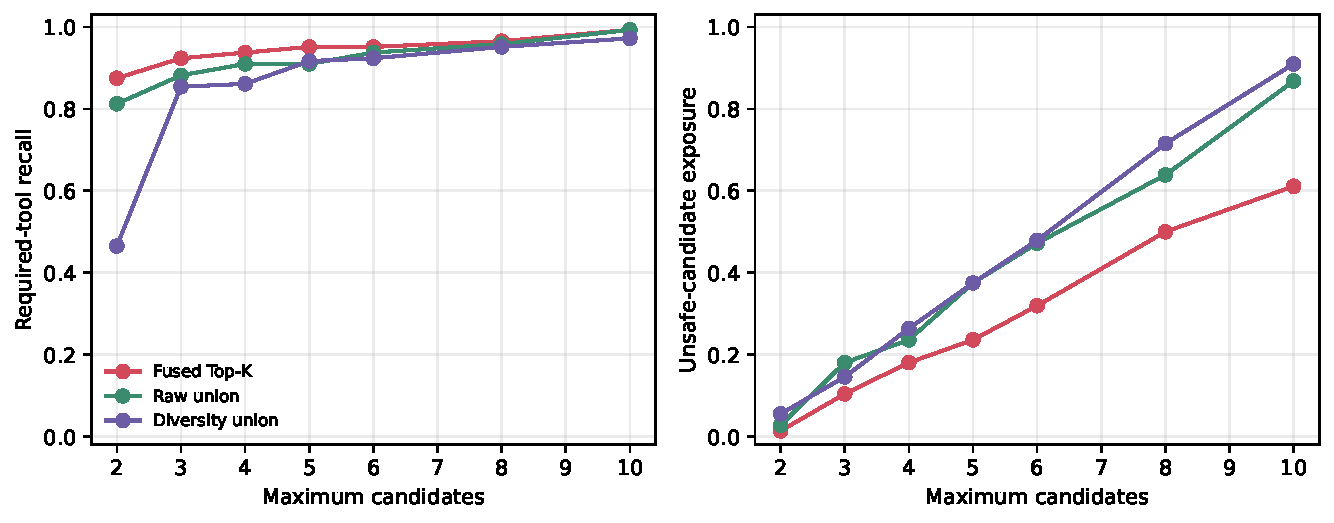
\includegraphics[width=.92\linewidth]{../shared/results/paper6_5_tools/auto_discovery_ablation/auto_union_vs_fusion.pdf}
\caption{A7 frozen-test frontier. Union does not dominate fused Top-K in
required-tool recall and raises unsafe-candidate exposure rapidly as the
palette grows. Discovery exposure is diagnostic; host authorization remains a
separate execution boundary.}
\label{fig:m8-auto-union}
\end{figure}

\subsection{Semantic confusion changes the large-catalog result}
M0 established that a typed index can locate opaque resources in catalogs up
to 8,192 entries. That result did not test whether zero-configuration semantic
channels preserve ranking quality when thousands of plausible callable
descriptions compete for the same intent. The scale follow-up therefore keeps
the 18 target callables and 144 frozen H0--H5 test requests, then constructs
catalogs of 32, 128, 512, 2,048, and 8,192 ordinary Python callables under five
catalog seeds. Each added callable shares exactly one canonical facet with a
target---its operation or its object---but never both. Names, docstrings,
signatures, annotations, and modules are inspectable by the same registration
path as the targets. Every fifth eligible distractor uses a destructive
operation on the anchor object so unsafe exposure remains measurable. No
generated distractor receives a manual tag or target label at ranking time.

The evaluation reruns A2 lexical-plus-synonym scoring, A5 compact embeddings,
A6 with the representation and weights frozen on the original 18-tool
validation set, and A7 equal fusion, raw union, and diversity union. Candidate
budgets $K\in\{2,3,4,5,6,8,10,20\}$ are matched exactly. Table~\ref{tab:m8-scale}
reports seed means at $K=10$; ``Union P'' is useful precision and ``Unsafe'' is
the fraction of requests whose candidate palette contains at least one labeled
destructive non-target. Exposure is diagnostic and never grants execution
authority.

\begin{table}[H]
\centering
\small
\resizebox{\linewidth}{!}{\begin{tabular}{rcccccccc}
\toprule
Catalog & A2 Top-1 & A5 Top-1 & A6 Top-1 & A6 R@10 & Union R & Union P & Unsafe & Tokens \\
\midrule
32 & 0.729 & 0.529 & 0.787 & 0.967 & 0.944 & 0.153 & 0.414 & 916 \\
128 & 0.629 & 0.394 & 0.675 & 0.914 & 0.879 & 0.120 & 0.399 & 1026 \\
512 & 0.564 & 0.272 & 0.546 & 0.850 & 0.801 & 0.101 & 0.208 & 1050 \\
2,048 & 0.472 & 0.229 & 0.421 & 0.692 & 0.715 & 0.085 & 0.125 & 1057 \\
8,192 & 0.451 & 0.206 & 0.338 & 0.553 & 0.662 & 0.078 & 0.110 & 1059 \\
\bottomrule
\end{tabular}
}
\caption{Five-seed semantically confusable callable-catalog scaling. A2--A6
columns report ranking quality. Union columns report raw A7 union at matched
$K=10$; context tokens serialize complete selected schemas.}
\label{tab:m8-scale}
\end{table}

The original frozen hybrid remains strongest at 32 and 128 tools. Its Top-1
advantage disappears by 512 and reverses at 2,048: at 8,192, A2 lexical
evidence reaches \PaperSixFiveScaleEightKLexicalTopOne{} Top-1 while A6 reaches
\PaperSixFiveScaleEightKHybridTopOne{}. The compact embedding alone falls to
.206. Semantic similarity accumulates plausible neighbors as the catalog
grows, whereas exact lexical evidence retains a sharper identity signal.
Figure~\ref{fig:m8-scale-quality} shows that this is a gradual ranking failure,
not a threshold artifact.

\begin{figure}[H]
\centering
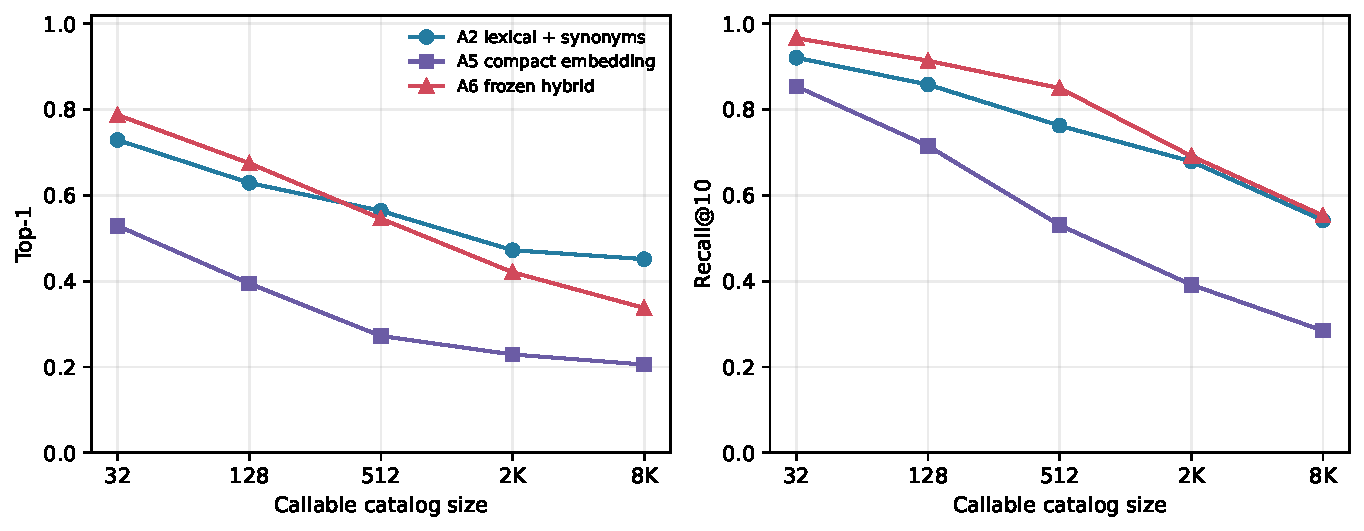
\includegraphics[width=.96\linewidth]{../shared/results/paper6_5_tools/auto_discovery_scaling/scaled_auto_quality.pdf}
\caption{Top-1 and Recall@10 under five seeded callable catalogs. The A6
mixture is frozen rather than retuned at each scale.}
\label{fig:m8-scale-quality}
\end{figure}

Channel diversity nevertheless becomes useful for bounded recovery. At 8,192
tools and $K=10$, raw union reaches
\PaperSixFiveScaleEightKUnionRecallTen{} required-tool recall, compared with
\PaperSixFiveScaleEightKHybridRecallTen{} for A6. The gain is not free: useful
precision is \PaperSixFiveScaleEightKUnionPrecisionTen{}, the palette exposes a
labeled unsafe candidate on \PaperSixFiveScaleEightKUnionUnsafeTen{} of
requests, and full schemas consume \PaperSixFiveScaleEightKUnionTokensTen{}
tokens on average. The declining unsafe-exposure rate with catalog size does
not imply safer catalogs; under fixed $K$, increasingly many non-destructive
confusable candidates displace destructive ones from the visible palette.
Figure~\ref{fig:m8-scale-union} therefore reports recall and exposure together.

\begin{figure}[H]
\centering
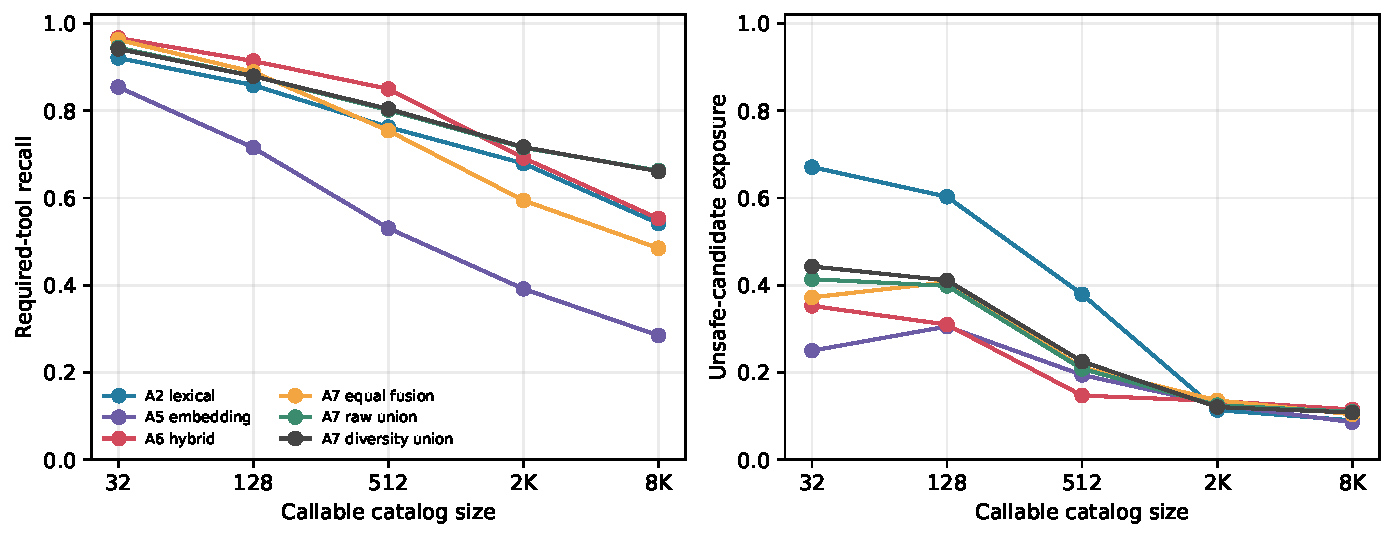
\includegraphics[width=.96\linewidth]{../shared/results/paper6_5_tools/auto_discovery_scaling/scaled_union_k10.pdf}
\caption{Matched-$K=10$ required-tool recall and unsafe-candidate exposure.
Raw and diversity union preserve more large-catalog recall, but neither is a
safe or precise default disclosure policy.}
\label{fig:m8-scale-union}
\end{figure}

Figure~\ref{fig:m8-scale-frontier} exposes the 8K budget tradeoff rather than
selecting $K=10$ after the fact. Union's recall advantage grows with palette
size while useful precision falls; $K=20$ is a diagnostic upper bound, not a
recommended disclosure budget.

\begin{figure}[H]
\centering
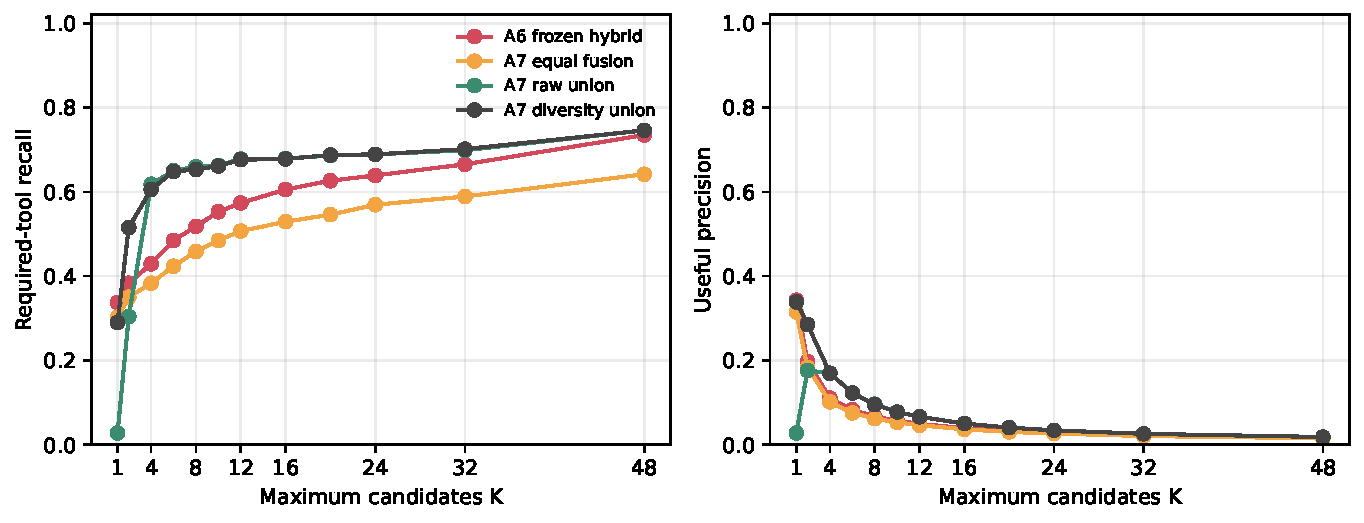
\includegraphics[width=.94\linewidth]{../shared/results/paper6_5_tools/auto_discovery_scaling/scaled_union_frontier_8192.pdf}
\caption{The 8,192-tool matched-budget frontier. Candidate-set recall and
useful precision must be read together.}
\label{fig:m8-scale-frontier}
\end{figure}

The Python reference implementation scales approximately linearly. At 8,192
tools, exhaustive BM25 scoring takes
\PaperSixFiveScaleEightKBMLatency{} ms/query and tensorized A7 candidate
construction takes \PaperSixFiveScaleEightKASevenLatency{} ms/query after
channel scores are available. Discovery components occupy
\PaperSixFiveScaleEightKMemoryMiB{} MiB, while serializing the entire logical
catalog would require \PaperSixFiveScaleEightKLogicalTokens{} tokens. These
measurements establish the cost shape, not a production latency claim: an
inverted lexical index and approximate semantic index should narrow candidates
before exact reranking.

\begin{figure}[H]
\centering
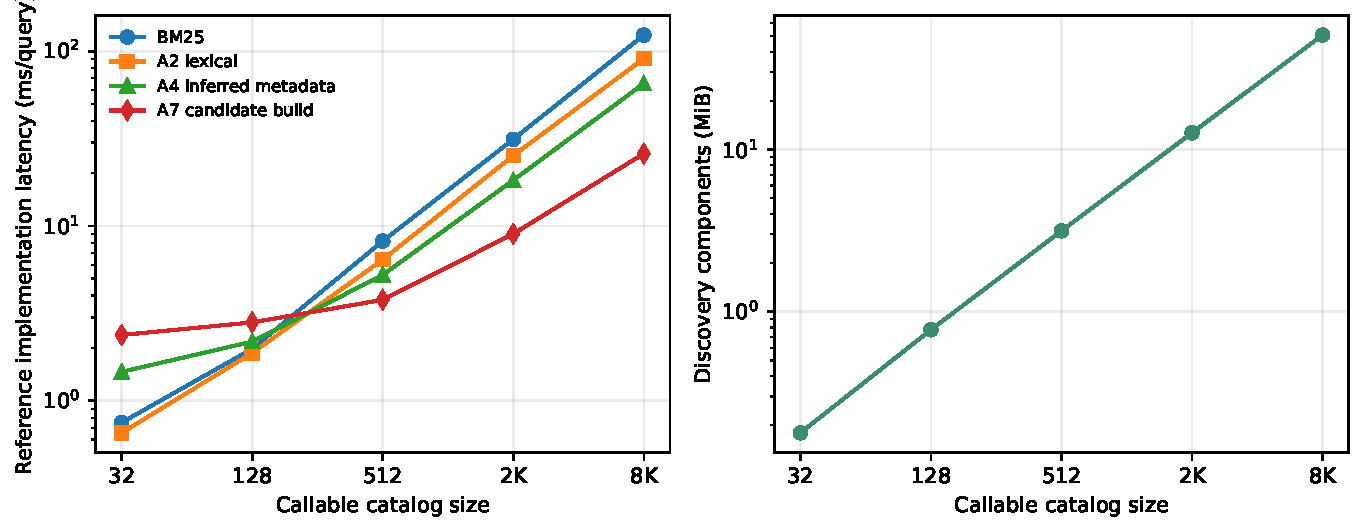
\includegraphics[width=.94\linewidth]{../shared/results/paper6_5_tools/auto_discovery_scaling/scaled_auto_costs.pdf}
\caption{Reference implementation latency and measured discovery-component
memory. Both axes are logarithmic; query encoding is batched and reported
separately in the machine-readable cost rows.}
\label{fig:m8-scale-cost}
\end{figure}

The large-catalog result reopens A7 only as a retrieval research direction.
It does not reopen the default-union or generative JIT gate because recall does
not dominate useful precision, safety exposure, and schema context jointly.
A production follow-up should use indexed candidate narrowing, calibrate
abstention at each catalog scale, and test whether a second-stage reranker can
retain the union's recall before any schema becomes model-visible.

\subsection{Selection authority and atomic tool records}
M8 separates selection from materialization. The agent resolver owns catalog
semantics, execution state, tenant and safety filters, and the candidate budget.
It emits an authoritative \texttt{TOOL\_CATALOG\_SLICE} whose children are
atomic \texttt{TOOL\_DEFINITION} records. PRA preserves child identity,
version, fingerprint, parent relation, field boundaries, and channel
provenance, then materializes every admitted child in full. It does not rerank
or prune chunks inside a selected schema.

If the slice exceeds the declared budget, the runtime must request a narrower
slice, return an error, use an explicitly allowed temporary expansion, or drop
whole records in candidate-priority order. Silent partial-schema fallback is
invalid. The same substrate can construct tool responses, logs, terminal
outputs, database results, and RAG chunks. M9 adds only predefined selection and
full views for capability records; dynamic field reduction and detail expansion
remain future work rather than hidden behavior in this paper.

E4 reruns the three frozen workflows across five prompt presentations with
Top-1 JIT, diversity-union JIT at $K=2,4,6,8$, static required-set and graph
sets, and all safe tools. The frozen Qwen3-0.6B Q4 model obtains
\PaperSixFiveTopOneJITSuccess{} strict task success at Top-1 and
\PaperSixFiveUnionKTwoSuccess{}, \PaperSixFiveUnionKFourSuccess{},
\PaperSixFiveUnionKSixSuccess{}, and \PaperSixFiveUnionKEightSuccess{} at the
four union budgets. All-tools reaches only \PaperSixFiveAllToolsSuccess{} despite
complete candidate recall. The prompt presentations are robustness conditions,
not training seeds; no model parameter changes. Figure~\ref{fig:m8-jit} and
Table~\ref{tab:m8-jit} report execution success against disclosure cost rather
than treating set recall as execution success.

\begin{table}[H]
\centering
\small
\begin{tabular}{lrrrr}
\toprule
Policy & Success & Required recall & Schema tokens & Disclosed tools \\
\midrule
Top-1 JIT & 0.000 & 0.857 & 191 & 2.3 \\
Union JIT, $K=2$ & 0.333 & 1.000 & 495 & 5.3 \\
Union JIT, $K=4$ & 0.333 & 1.000 & 964 & 6.9 \\
Union JIT, $K=6$ & 0.400 & 1.000 & 1371 & 9.2 \\
Union JIT, $K=8$ & 0.600 & 1.000 & 1922 & 11.8 \\
Static required-set oracle & 0.267 & 1.000 & 839 & 4.0 \\
Static graph set & 0.133 & 1.000 & 1337 & 8.0 \\
All tools & 0.133 & 1.000 & 2411 & 17.0 \\
\bottomrule
\end{tabular}

\caption{E4 aggregate over 15 workflows per policy. Schema tokens are cumulative
over attempted JIT steps; disclosed tools count unique definitions per workflow.}
\label{tab:m8-jit}
\end{table}

\begin{figure}[H]
\centering
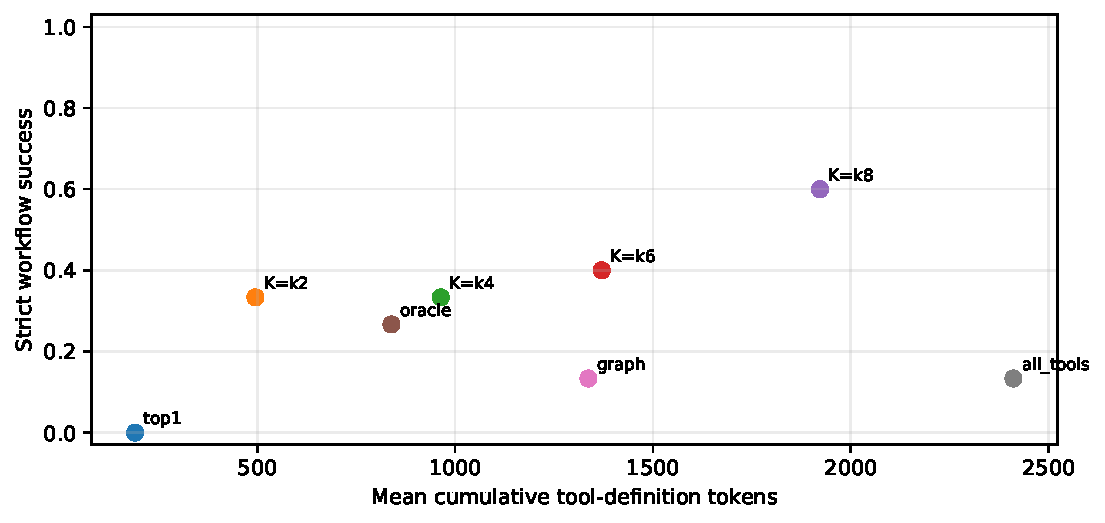
\includegraphics[width=.86\linewidth]{../shared/results/paper6_5_tools/auto_union_records/union_jit_frontier.pdf}
\caption{E4 strict workflow success against cumulative visible schema tokens.
The frozen model, host authorization, and pure handlers are unchanged across
candidate policies.}
\label{fig:m8-jit}
\end{figure}

E5--E6 compare provider-structured full records, flat textual serialization,
parameters without a description, descriptions without parameters, and a
schema with one required field deliberately removed. Across 20 calls per
condition, full atomic records obtain \PaperSixFiveAtomicCallValidity{} accepted
execution. Parameter-bearing structured records also reach 1.000 on these simple
single-step calls, while description-only records reach
\PaperSixFiveDescriptionOnlyValidity{}. An explicit content-only internal-chunk
router, which selects either the description or parameter-schema segment,
likewise reaches only \PaperSixFiveGenericChunkValidity{}. Dropping one required
field lowers acceptance to
\PaperSixFiveDroppedFieldValidity{} and causes required-argument omission at
rate \PaperSixFiveDroppedFieldOmission{}. These controls support full selected-
tool materialization as the default. M9 retains that atomic full view after
selection; it does not introduce progressive detail expansion inside a schema.

\begin{figure}[H]
\centering
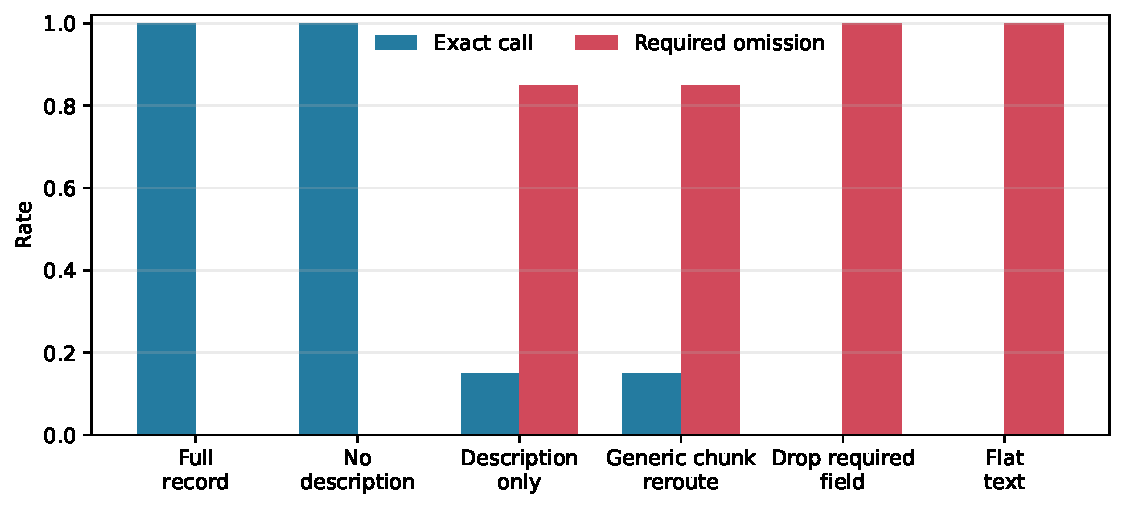
\includegraphics[width=.88\linewidth]{../shared/results/paper6_5_tools/auto_union_records/tool_atomicity_controls.pdf}
\caption{E5--E6 exact calls and required-argument omissions. The generic router
selects one internal schema segment; all partial-schema conditions are
experimental controls, not runtime fallback policies.}
\label{fig:m8-atomic}
\end{figure}

\section{M9: Typed Progressive Disclosure}

Tool and skill records require different detail during choice and use. A model
can often choose between capabilities from identity, signature or applicability,
and a short description. It needs the complete parameter schema only when
constructing a call, and the complete instruction body only when applying a
skill. M9 represents this distinction as two deterministic views of one typed,
versioned record:
\[
R_{\mathrm{select}}\longrightarrow R_{\mathrm{full}}.
\]
This transition is not token truncation or learned summarization. Field
selection is defined by record type, and both views remain semantic record
units. A full view is admitted atomically or not at all.

\subsection{Records and explicit two-phase execution}

A tool selection view contains stable name, call signature, short description,
and side-effect class. Its full view contains the complete nested input schema,
required and optional fields, enums and defaults, return schema, identity,
version, and authorization-relevant metadata. A declarative skill selection
view contains name, description, and when-to-use text. Its full view additionally
contains ordered instructions, constraints, examples, dependencies, references,
namespace, tenant, and version metadata. M9 supports text-only skills; it rejects
script or executable payload metadata.

The runtime performs two ordinary model invocations. Phase A materializes the
selection view of every externally bounded candidate and requests one structured
capability identity. A validated \texttt{CapabilityTransition} permits only
\texttt{selection}$\rightarrow$\texttt{full}. Phase B removes non-selected
candidates, materializes the selected full record, and asks the model to produce
arguments or follow the selected instructions. Discovery and materialization do
not grant execution authority; the existing host validator still checks selected
identity, schema, side-effect policy, and request-scoped authorization.

The implementation is deliberately simple. Named views and policy validation
live in \path{src/pra_hf/context_records.py}; the transition and token/KV
accounting live in \path{src/pra_hf/progressive_disclosure.py}; and declarative
skill records live in \path{src/pra_hf/skill_records.py}. There is no generation
callback, decoder interruption, confidence-triggered expansion, arbitrary
compression, or mid-token materialization. Those dynamic mechanisms belong to
a later large-record study.

For candidate full-view tokens $F_K$, Phase-A selection tokens $A_K$, and the
selected full-view tokens $B$, we report
\[
  \mathrm{DisclosureRatio}=\frac{A_K}{F_K},\qquad
  \mathrm{TotalDisclosureRatio}=\frac{A_K+B}{F_K}.
\]
The latter counts both model phases and therefore does not hide the second
invocation.

\subsection{Protocol}

The tool experiment freezes \PaperSixFiveMNineToolCases{} semantic-hard requests
over the 18 M8 callables. The skill benchmark contains
\PaperSixFiveMNineSkillCatalog{} realistic, semantically confusable declarative
skills and 50 name-blind requests split evenly between validation and test.
Validation selects the same external BM25, automatic semantic, compact-embedding,
and fused discovery stack used for tools. Generation uses
\PaperSixFiveMNineSkillCases{} held-out skill requests. Both experiments compare
full-all (T0/S0), selection-only (T1/S1), selection-to-full (T2/S2), and
oracle-full (T3/S3). Tool budgets retain the original bounded-palette grid;
skills use $K\in\{2,4,8,16,24,32\}$ over the 50-record catalog.

All generation rows use the exact frozen Qwen3-0.6B revision in FP16 on an
NVIDIA GeForce GTX 950M, deterministic decoding, and no parameter updates. The
small eight-request generation cohorts are mechanism checks, not population
estimates. Tool evaluation separates required Recall@$K$, capability choice,
schema validity, argument semantics, host acceptance, and strict success. Skill
evaluation uses deterministic identity markers, required output headings, and
forbidden external-action claims. Timing includes CUDA synchronization,
serialization, both TTFTs, and both generations.

\subsection{Discovery and view size}

The shared discovery stack transfers without a second skill-specific retrieval
system. On the 50-query skill test split, BM25 obtains
\PaperSixFiveMNineSkillBmTwentyTopOne{} Top-1, compact embeddings obtain 0.800,
and validation-selected fusion obtains \PaperSixFiveMNineSkillFusedTopOne{}.
Fused Recall@$K$ rises from 0.840 at $K=2$ to 0.940 at $K=4$, 0.960 at
$K=8$, and 1.000 at $K=16$.
The corresponding tool bars in Figure~\ref{fig:m9-discovery} reuse M8's 144
test requests and should not be read as a paired cross-type comparison.

\begin{figure}[H]
\centering
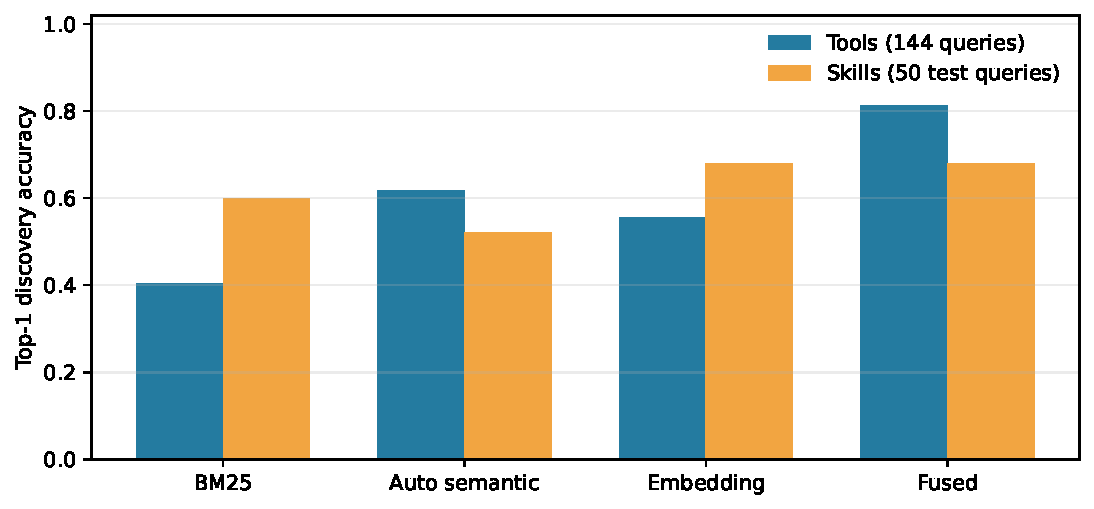
\includegraphics[width=.82\linewidth]{../shared/results/paper6_5_tools/progressive_disclosure/capability_discovery_generalization.pdf}
\caption{The same external discovery families applied to tools and declarative
skills. Cohort sizes differ; the figure tests substrate reuse, not which
resource type is intrinsically easier.}
\label{fig:m9-discovery}
\end{figure}

Full tool schemas contain a median 233.5 tokens (p95 244), and their selection
views retain a median 0.368 of that count. Full skill instructions contain a
median 685 tokens (p95 1,353), while skill selection views retain 0.150. These
bodies are intentionally nontrivial: full-all instruction cost therefore grows
linearly with the candidate palette.

\begin{figure}[H]
\centering
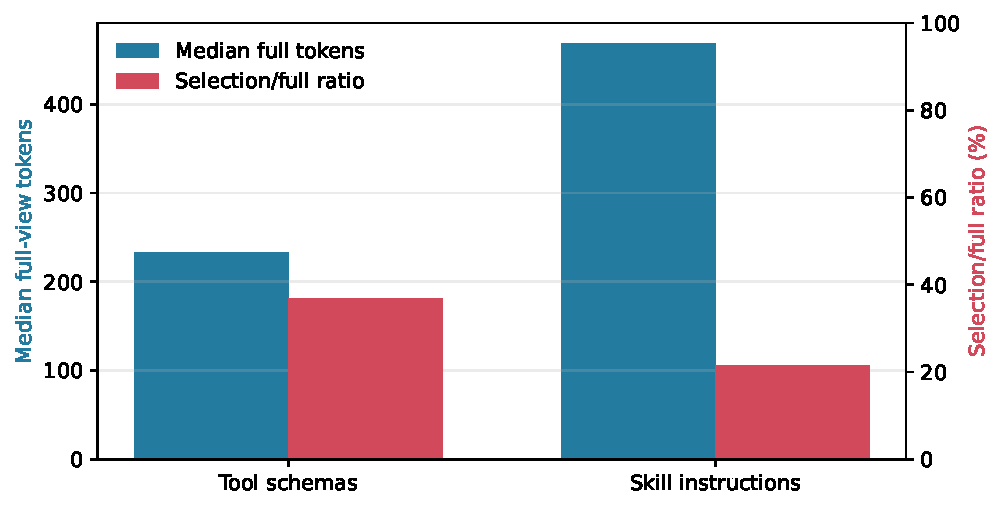
\includegraphics[width=.72\linewidth]{../shared/results/paper6_5_tools/progressive_disclosure/capability_view_size_distribution.pdf}
\caption{Median full-view tokens and median selection/full token ratio for the
18 tool schemas and 50 declarative skills. Ratios are percentages in the red
bars; no view is formed by first-$N$-token truncation.}
\label{fig:m9-view-size}
\end{figure}

\begin{table}[H]
\centering
\scriptsize
\resizebox{\linewidth}{!}{\begin{tabular}{lrrrrrrrr}
\toprule
Bucket & $n$ & Instr. & Select & Full & Saved & R@8 & Choice & Success \\
\midrule
Short & 17 & 177 & 103 & 510 & 0.78 & 0.88 & 0.00 & 0.00 \\
Medium & 17 & 345 & 103 & 687 & 0.78 & 1.00 & 0.00 & 0.00 \\
Long & 16 & 972 & 104 & 1341 & 0.70 & 1.00 & 1.00 & 1.00 \\
\bottomrule
\end{tabular}
}
\caption{Skill results by measured instruction-length bucket. Token columns are
means; ``Saved'' is the mean $K=8$ progressive token saving. Choice and success
come from four stratified generation cases (two short, one medium, one long),
so they are mechanism diagnostics rather than bucket-level estimates.}
\label{tab:skill-length}
\end{table}

\subsection{Tools: choice improves at moderate budgets, not at catalog scale}

Table~\ref{tab:m9-tools} reports the full tool matrix. At $K=4$, T2 raises
choice accuracy from \PaperSixFiveMNineToolKFourFullChoice{} to
\PaperSixFiveMNineToolKFourProgressiveChoice{} and strict success from
\PaperSixFiveMNineToolKFourFullSuccess{} to
\PaperSixFiveMNineToolKFourProgressiveSuccess{}, while exposing
\PaperSixFiveMNineToolKFourDisclosure{} of T0's capability tokens. At $K=8$,
T0 and T2 both obtain \PaperSixFiveMNineToolKEightProgressiveChoice{} choice
accuracy; T2 uses \PaperSixFiveMNineToolKEightDisclosure{} of full-all tokens
but adds \PaperSixFiveMNineToolKEightWallOverhead{} seconds mean wall time.
At all 18 tools, T2 choice falls to 0.375 versus 0.625 for T0. Compact views do
not remove the need for bounded discovery.

\begin{table}[!t]
\centering
\scriptsize
\resizebox{\linewidth}{!}{\begin{tabular}{rrl r@{\hspace{1.1em}}r@{\hspace{1.1em}}r@{\hspace{1.1em}}r@{\hspace{1.1em}}r@{\hspace{1.1em}}r}
\toprule
$K$ & $n$ & Condition & Recall & Choice & Valid/follow & Success & Tokens & Wall (s) \\
\midrule
2 & 8 & T0 full-all & 0.88 & 0.75 & 0.88 & 0.50 & 472.00 & 4.36 \\
2 & 8 & T1 selection-only & 0.88 & 0.00 & 0.00 & 0.00 & 173.88 & 2.93 \\
2 & 8 & T2 select$\rightarrow$full & 0.88 & 0.75 & 0.88 & 0.25 & 381.88 & 5.00 \\
2 & 8 & T3 oracle-full & 0.88 & 1.00 & 1.00 & 0.38 & 236.88 & 4.04 \\
\addlinespace
4 & 8 & T0 full-all & 1.00 & 0.50 & 0.88 & 0.25 & 945.50 & 4.63 \\
4 & 8 & T1 selection-only & 1.00 & 0.00 & 0.00 & 0.00 & 349.12 & 2.88 \\
4 & 8 & T2 select$\rightarrow$full & 1.00 & 0.88 & 0.88 & 0.38 & 557.12 & 5.43 \\
4 & 8 & T3 oracle-full & 1.00 & 1.00 & 1.00 & 0.38 & 236.88 & 4.06 \\
\addlinespace
6 & 8 & T0 full-all & 1.00 & 0.62 & 1.00 & 0.25 & 1417.00 & 4.96 \\
6 & 8 & T1 selection-only & 1.00 & 0.00 & 0.00 & 0.00 & 523.62 & 3.31 \\
6 & 8 & T2 select$\rightarrow$full & 1.00 & 0.75 & 1.00 & 0.25 & 759.88 & 6.42 \\
6 & 8 & T3 oracle-full & 1.00 & 1.00 & 1.00 & 0.38 & 236.88 & 4.08 \\
\addlinespace
8 & 8 & T0 full-all & 1.00 & 0.62 & 0.88 & 0.38 & 1889.25 & 5.75 \\
8 & 8 & T1 selection-only & 1.00 & 0.00 & 0.00 & 0.00 & 697.88 & 3.44 \\
8 & 8 & T2 select$\rightarrow$full & 1.00 & 0.62 & 0.88 & 0.12 & 904.50 & 6.25 \\
8 & 8 & T3 oracle-full & 1.00 & 1.00 & 1.00 & 0.38 & 236.88 & 3.92 \\
\addlinespace
18 & 8 & T0 full-all & 1.00 & 0.62 & 0.88 & 0.38 & 4235.00 & 8.49 \\
18 & 8 & T1 selection-only & 1.00 & 0.00 & 0.00 & 0.00 & 1567.00 & 8.55 \\
18 & 8 & T2 select$\rightarrow$full & 1.00 & 0.38 & 0.62 & 0.00 & 1715.12 & 8.85 \\
18 & 8 & T3 oracle-full & 1.00 & 1.00 & 1.00 & 0.38 & 236.88 & 4.06 \\
\bottomrule
\end{tabular}
}
\caption{Tool progressive-disclosure matrix. $n$ is the number of context-fitting
generation cases. ``Valid/follow'' is schema-valid call rate. Strict success
also requires the exact benchmark arguments and accepted host execution.}
\label{tab:m9-tools}
\end{table}

Selection-only obtains no strict successes: compact signatures are sufficient
for choosing in some rows, but are not a reliable replacement for full provider
schemas during argument construction. T3 obtains 1.000 schema validity and host
acceptance at every budget, yet only 0.375 strict success because five of eight
requests elicit non-exact argument values even when the correct tool is supplied
alone. This oracle ceiling is why M9 does not interpret low strict success as a
routing-only failure.

\subsection{Skills: context economy under a bounded candidate set}

At $K=8$, the full-all condition does not fit the declared 8,192-token runtime
limit for any of the four stratified generation cases. Selection-to-full fits
all four while exposing 0.300 of full-all capability tokens. It chooses and
applies the correct skill in one case (0.250 strict success); oracle-full
obtains 1.000. S1 fails the required identity and output contract throughout,
confirming that compact applicability text is a choice surface rather than a
replacement for the authoritative instructions. The four-case cohort is a
mechanism check: it establishes feasibility and exposes the remaining choice
error, but it is too small for a population-level quality claim.

\clearpage
\begin{table}[H]
\centering
\scriptsize
\resizebox{\linewidth}{!}{\begin{tabular}{rrl r@{\hspace{1.1em}}r@{\hspace{1.1em}}r@{\hspace{1.1em}}r@{\hspace{1.1em}}r@{\hspace{1.1em}}r}
\toprule
$K$ & $n$ & Condition & Recall & Choice & Valid/follow & Success & Tokens & Wall (s) \\
\midrule
2 & 8 & S0 full-all & 0.88 & 0.75 & 0.88 & 0.62 & 921.38 & 13.11 \\
2 & 8 & S1 selection-only & 0.88 & 0.00 & 0.00 & 0.00 & 199.88 & 6.78 \\
2 & 8 & S2 select$\rightarrow$full & 0.88 & 0.62 & 0.88 & 0.62 & 602.62 & 11.33 \\
2 & 8 & S3 oracle-full & 0.88 & 1.00 & 1.00 & 1.00 & 460.62 & 11.27 \\
\addlinespace
4 & 8 & S0 full-all & 0.88 & 0.75 & 1.00 & 0.75 & 1852.62 & 24.79 \\
4 & 8 & S1 selection-only & 0.88 & 0.00 & 0.00 & 0.00 & 402.38 & 9.36 \\
4 & 8 & S2 select$\rightarrow$full & 0.88 & 0.62 & 0.88 & 0.62 & 805.00 & 12.74 \\
4 & 8 & S3 oracle-full & 0.88 & 1.00 & 1.00 & 1.00 & 460.62 & 11.06 \\
\addlinespace
6 & 8 & S0 full-all & 0.88 & 0.75 & 0.88 & 0.62 & 2794.00 & 34.74 \\
6 & 8 & S1 selection-only & 0.88 & 0.00 & 0.00 & 0.00 & 606.62 & 9.60 \\
6 & 8 & S2 select$\rightarrow$full & 0.88 & 0.50 & 0.75 & 0.50 & 1067.12 & 15.91 \\
6 & 8 & S3 oracle-full & 0.88 & 1.00 & 1.00 & 1.00 & 460.62 & 11.01 \\
\addlinespace
8 & 8 & S0 full-all & 1.00 & 0.62 & 1.00 & 0.62 & 3728.75 & 63.87 \\
8 & 8 & S1 selection-only & 1.00 & 0.00 & 0.00 & 0.00 & 808.25 & 10.40 \\
8 & 8 & S2 select$\rightarrow$full & 1.00 & 0.62 & 0.88 & 0.62 & 1269.88 & 15.90 \\
8 & 8 & S3 oracle-full & 1.00 & 1.00 & 1.00 & 1.00 & 460.62 & 11.15 \\
\addlinespace
25 & 0 & S0 full-all & 1.00 & -- & -- & -- & -- & -- \\
25 & 8 & S1 selection-only & 1.00 & 0.00 & 0.00 & 0.00 & 2527.00 & 33.70 \\
25 & 8 & S2 select$\rightarrow$full & 1.00 & 0.50 & 0.75 & 0.50 & 2928.50 & 23.98 \\
25 & 8 & S3 oracle-full & 1.00 & 1.00 & 1.00 & 1.00 & 460.62 & 11.16 \\
\bottomrule
\end{tabular}
}
\caption{Declarative-skill progressive-disclosure matrix. ``Valid/follow'' is
deterministic instruction-contract success. Quality $n$ counts rows that fit
the runtime envelope. Full-all has no fitting rows from $K=8$ onward. Three
$K=32$ rows per executable condition completed; the fourth stalled during the
long selection prompt and is reported as missing, not imputed.}
\label{tab:m9-skills}
\end{table}

At $K=32$, full-all would expose 26,094 mean capability tokens and cannot run
under the measured GPU limit. Selection-to-full exposes 4,658 tokens in the
three completed rows and obtains 0.333 strict success. Because one stratified
case is absent, the $K=32$ value is descriptive only. This stress result
establishes feasibility under one hardware envelope; it does not imply that
larger-memory runtimes cannot execute full-all.

\begin{figure}[H]
\centering
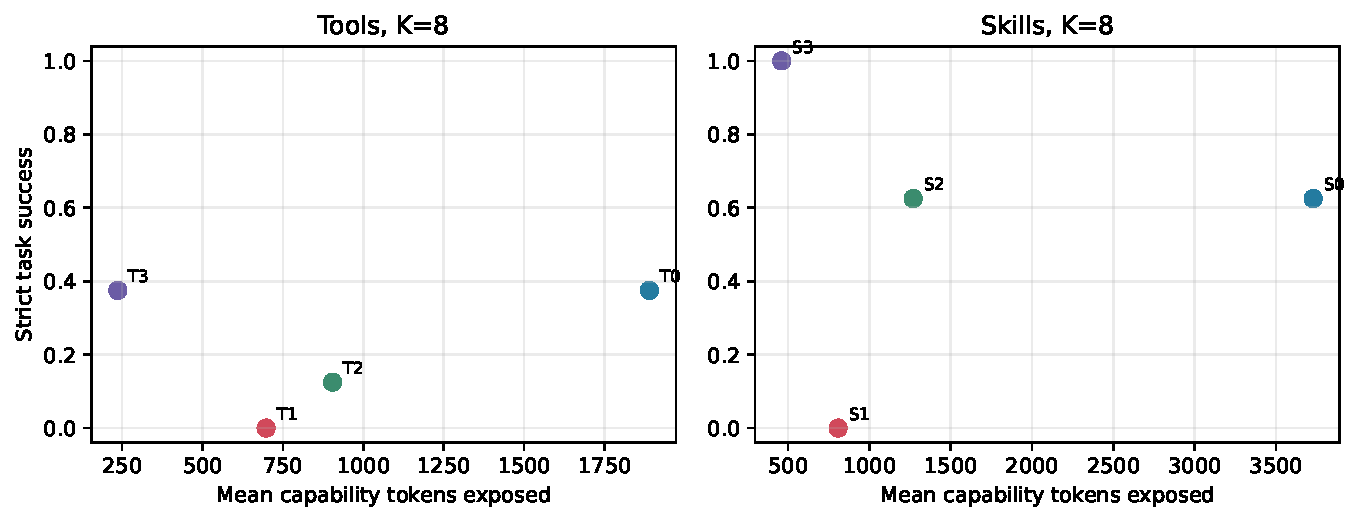
\includegraphics[width=.90\linewidth]{../shared/results/paper6_5_tools/progressive_disclosure/progressive_disclosure_pareto.pdf}
\caption{Strict task success against total capability tokens exposed at $K=8$.
Totals include both phases for T2/S2. The oracle points isolate the call or
instruction-following ceiling after externally correct selection.}
\label{fig:m9-pareto}
\end{figure}

\subsection{Gate decision}

The architectural gate opens: typed selection/full views, explicit transitions,
atomic selected records, and shared tool/skill discovery work without callback
machinery. The skill inclusion gate also opens because fused discovery exceeds
BM25 by 0.160 Top-1 and selected-full execution cuts instruction context while
remaining deterministically evaluable. The deployment gate is conditional.
Selection-to-full is the SDK policy for an already bounded capability palette,
but the resolver must retain its calibrated candidate limit and host safety
checks. This small cohort does not establish statistical non-inferiority, and
the all-tool result rejects using compact views as a substitute for discovery.

\section{M10: Large-Catalog Palette Use}

The 8,192-tool retrieval result leaves a downstream question open. A larger
candidate set is useful only when the model can identify the target among its
additional confusable tools. M10 freezes the same callable generator and eight
M9 tool requests, then separates three probabilities:
\[
P(t\in C),\qquad P(\hat t=t\mid t\in C),\qquad P(\hat t=t).
\]
The first is resolver recall, the second is model discrimination conditional
on a successful resolver, and the third is their end-to-end product. Every raw
row retains the chosen identity, candidate count, channel sources and ranks,
unsafe and useful candidates, view tokens, and wall time.

\subsection{Protocol and model boundary}

The base retrieval grid covers $N\in\{32,128,512,2048,8192\}$,
$K\in\{2,4,6,8,10\}$, and BM25, frozen fusion, raw union, and diversity union.
Seed 11 covers the Cartesian grid. The decisive $N=8192,K=10$ comparison uses
all five catalog seeds and 40 query--seed pairs; a fixed agreement bonus is an
additional control. A targeted diversity-only extension evaluates
$K\in\{12,16,24,32\}$ on those same 40 pairs. Target-absent palettes are
recorded without calling the chooser, because their end-to-end outcome is
already determined; target-present palettes use the identical frozen chooser.
Candidate identities are bound to labels and the official Ollama
\texttt{qwen3:0.6b} Q4 artifact generates one label at temperature zero. This
low-memory artifact is kept separate from the exact FP16 CUDA model used below
for call construction. Catalog seeds vary generated distractors, not model
weights.

The 40-row recall values in Table~\ref{tab:m10-palette} differ from the
144-query values in Table~\ref{tab:m8-scale} because M10 uses the smaller
argument-annotated generation cohort. They answer different questions: M8
estimates resolver behavior on all frozen test requests; M10 tests whether a
model can use selected palettes on requests with executable expected calls.

\begin{figure}[H]
\centering
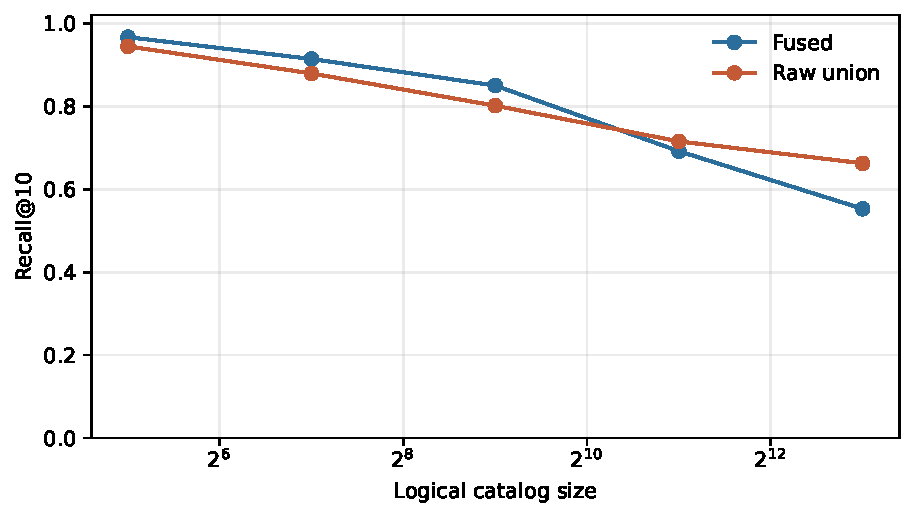
\includegraphics[width=.82\linewidth]{../shared/results/paper6_5_tools/missing_experiments/large_n_retrieval_frontier.pdf}
\caption{Five-seed large-catalog Recall@10. Union increasingly helps candidate
generation as the logical catalog grows, before any candidate is shown to the
generation model.}
\label{fig:m10-retrieval}
\end{figure}

\subsection{Candidate recall is not candidate use}

\begin{table}[H]
\centering
\scriptsize
\resizebox{\linewidth}{!}{\begin{tabular}{lrrrrrr}
\toprule
Policy & $n$ & Recall & Cond. choice & End-to-end & Unsafe choice & Tokens \\
\midrule
BM25 & 40 & 0.375 & 0.600 & 0.225 & 0.000 & 1465 \\
Fused & 40 & 0.300 & 0.083 & 0.025 & 0.075 & 1514 \\
Raw union & 40 & 0.375 & 0.000 & 0.000 & 0.000 & 1464 \\
Diversity union & 40 & 0.375 & 0.667 & 0.250 & 0.000 & 1465 \\
Agreement union & 40 & 0.375 & 0.467 & 0.175 & 0.050 & 1464 \\
\bottomrule
\end{tabular}
}
\caption{Generated capability choice at $N=8192,K=10$ across eight requests
and five catalog seeds. Conditional choice excludes target-absent rows;
end-to-end choice counts them as failures. Tokens expose compact selection
views only.}
\label{tab:m10-palette}
\end{table}

Raw union raises recall from 0.300 for frozen fusion to 0.375, but Qwen chooses
none of its 15 available targets. The model cannot use raw union's additional
hypotheses. Diversity union retains the same 0.375 recall and chooses 10/15
available targets, yielding 0.250 end-to-end choice. Fusion obtains 1/12 and
0.025 respectively. On paired query--seed identities, diversity wins ten rows
that fusion loses and loses one row that fusion wins (exact two-sided
$p=0.0117$). The fixed agreement bonus obtains 7/15 conditional successes; its
paired effect versus fusion is unresolved ($p=0.0703$). This is evidence for
candidate ordering and channel diversity, not for broad schema disclosure.

\begin{figure}[H]
\centering
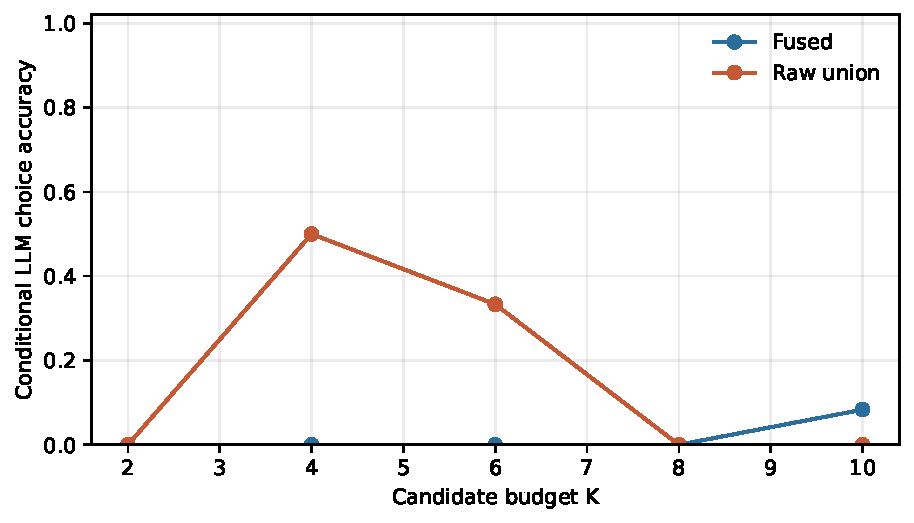
\includegraphics[width=.82\linewidth]{../shared/results/paper6_5_tools/missing_experiments/large_catalog_palette_use.pdf}
\caption{Conditional model choice across candidate budgets. A resolver gain
becomes operational only when the model can distinguish target from admitted
distractors.}
\label{fig:m10-palette-use}
\end{figure}

The compact/full view control uses 128 matched decisions over four stratified
requests. Compact views average 0.453 of full-view tokens and obtain 10/128
correct choices, versus 7/128 for full views. Both rates are low and this study
does not claim non-inferiority. It shows that exposing every nested schema field
does not repair large-catalog selection for this small model. Three executable
large-schema controls contain nested dataclasses, lists, optional objects,
enums, literals, and multiple required fields; their full views contain a
median 721 tokens (maximum 736), while selection views retain 0.219--0.279.

\subsection{Selection to atomic execution}

The causal execution matrix returns to the exact frozen Qwen3-0.6B FP16
revision. At $N=8192$ and $K\in\{4,8\}$, all five catalog seeds and four
requests compare full-all, compact-only, compact-to-full, and oracle-to-full.
The model first selects from complete compact records. The runtime then removes
losing records, materializes one full schema atomically, asks for arguments,
and submits the result to the same host validator. No resolver score grants
execution authority.

\begin{table}[H]
\centering
\scriptsize
\resizebox{\linewidth}{!}{\begin{tabular}{llrrrrr}
\toprule
Policy & View & Recall & Choice & Accepted & Strict & Tokens \\
\midrule
Fused & Full-all & 0.300 & 0.100 & 0.750 & 0.100 & 2615 \\
Fused & Select$\to$full & 0.300 & 0.100 & 0.650 & 0.100 & 1495 \\
Fused & Oracle full & 0.300 & 1.000 & 1.000 & 0.750 & 278 \\
Raw union & Full-all & 0.250 & 0.150 & 0.700 & 0.150 & 2561 \\
Raw union & Select$\to$full & 0.250 & 0.050 & 0.600 & 0.050 & 1441 \\
Raw union & Oracle full & 0.250 & 1.000 & 1.000 & 0.750 & 278 \\
Diversity union & Full-all & 0.250 & 0.000 & 0.500 & 0.000 & 2558 \\
Diversity union & Select$\to$full & 0.250 & 0.250 & 0.550 & 0.250 & 1419 \\
Diversity union & Oracle full & 0.250 & 1.000 & 1.000 & 0.750 & 278 \\
\bottomrule
\end{tabular}
}
\caption{Exact-FP16 large-catalog tool execution at $N=8192,K=8$ ($n=20$ per
row). Strict success requires target choice, exact benchmark arguments, and
accepted host execution. Oracle full isolates post-selection call quality.}
\label{tab:m10-progressive}
\end{table}

Diversity compact-to-full recovers every target-present row (5/5), obtains
5/20 strict accepted calls, and exposes 1,419 capability tokens on average,
0.556 of its 2,558-token full-all palette. It materializes one full schema and
avoids 2,294 full-schema tokens. Measured native-K/V accounting falls from
293.4 MB-equivalent bytes for full-all to 162.7 MB-equivalent bytes. Raw union
obtains 1/20 strict calls and fused obtains 2/20. Diversity versus fusion has
the same positive direction in 4 versus 1 discordant rows, but the 20-pair
effect is unresolved (exact $p=0.375$). Oracle-to-full obtains 15/20 strict
calls, locating the remaining ceiling in discovery and model choice rather
than schema execution alone.

\begin{figure}[H]
\centering
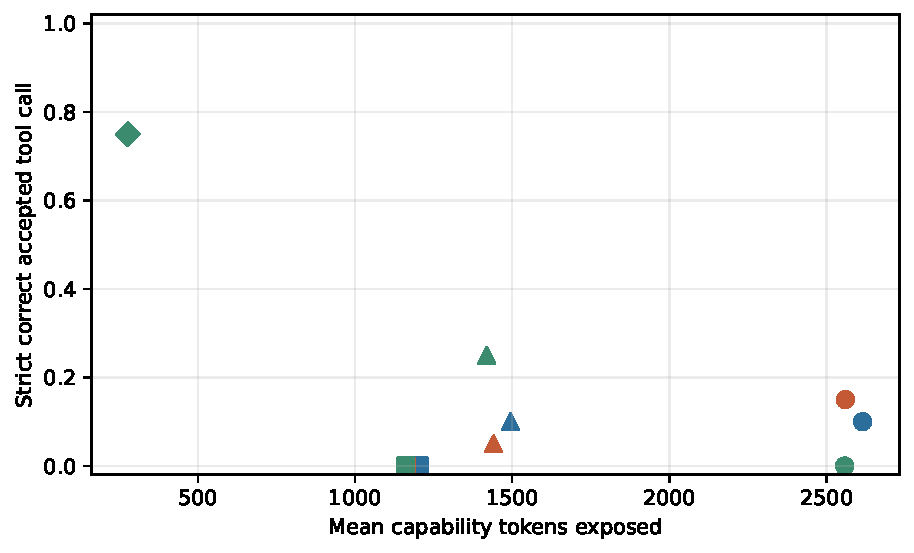
\includegraphics[width=.82\linewidth]{../shared/results/paper6_5_tools/missing_experiments/large_catalog_progressive_pareto.pdf}
\caption{Large-catalog strict accepted calls against total capability tokens
at $N=8192,K=8$. Two-phase totals include compact selection views and the one
selected full schema.}
\label{fig:m10-pareto}
\end{figure}

\subsection{Large-catalog JIT remains recall-bound}

Two two-step workflows pair account retrieval with update and document search
with export. For each step the resolver searches the full 8,192-tool logical
catalog, exposes $K\in\{4,8\}$ compact records, materializes one selected full
schema, validates the call, records a typed observation, and advances. The
five catalog seeds yield ten workflows per policy.

\begin{table}[H]
\centering
\scriptsize
\resizebox{\linewidth}{!}{\begin{tabular}{lrrrrrr}
\toprule
Policy & Steps & Recall & Cond. choice & Accepted & Workflow & Tokens \\
\midrule
Fused & 20 & 0.300 & 0.333 & 0.650 & 0.000 & 1495 \\
Raw union & 20 & 0.250 & 0.200 & 0.600 & 0.000 & 1441 \\
Diversity union & 20 & 0.250 & 1.000 & 0.550 & 0.000 & 1419 \\
\bottomrule
\end{tabular}
}
\caption{Large-catalog two-step JIT at $K=8$. Conditional choice can be high
while workflow success remains zero when a required step is absent from the
palette.}
\label{tab:m10-jit}
\end{table}

Diversity union again uses its successful palettes well: it chooses 5/5
target-present steps. But per-step recall is only 0.250, so no policy completes
either required step in all ten workflows. Raw union and fusion also obtain
zero workflow success. No generated proposal is an unsafe tool, but host
acceptance remains 0.55--0.65 because wrong identities and malformed or
incomplete arguments are still rejected. The default-union gate therefore
remains closed. The supported policy is frozen fusion by default, with
diversity union exposed as an experimental high-recall mode and explicit host
authorization after every selection.

\section{Deferred External Validations}
Work outside this paper returns to the broader persistent-context thesis: hierarchical
skills, mutation and revocation, bounded \texttt{\#\_\_head} history,
superseded facts, and permission-scoped child sessions
\[
M_{\mathrm{child}}=R(M_{\mathrm{parent}})\cup\Delta M_{\mathrm{child}}.
\]
Cross-model replication is also required because M2--M10 use one Qwen model
family for pretrained mechanisms and downstream capability choice. The
generated large-catalog study does not replace natural catalogs or a
tool-identity-disjoint benchmark;
both should test whether the observed lexical advantage and union recovery
survive distribution shift. The OpenAI-compatible endpoint belongs after these
mechanism checks, so harness behavior does not hide resolver, disclosure, or
execution failures.

\section{Reproducibility}
M8's E1--E3 driver is \path{run_auto_union_records.py}. Candidate sets for E4
are frozen by \path{run_union_jit_records.py} with
\texttt{--prepare-only}. The five-presentation E4--E6 driver is
\path{run_union_jit_ollama.py}. It uses the official
\texttt{qwen3:0.6b} Q4\_K\_M artifact on CPU with temperature zero, no GPU
offload, per-call unloading, and deterministic host-side schema validation.
This low-memory runtime is separate from the exact-FP16 M2--M7 rows. The runner
checkpoints at each completed condition. The companion summarizer regenerates
tables, macros, findings, and all four M8 figures.

The zero-configuration source, type, quality, and A0--A7 channel ablations use
\path{run_auto_discovery_ablation.py};
\path{summarize_auto_discovery_ablation.py} regenerates its table, macros, four
figures, and machine-readable summary. The driver constructs one frozen record
for each of the same 18 callables, selects embedding representation and fusion
weights only on validation, and evaluates all reported policies on 144 test
requests. It used the compact BGE encoder on an NVIDIA GeForce GTX 950M and
completed in 103 seconds. The manifest records every automatic field's source.
The A7 JIT status is a checked-in gate-closed artifact because no union condition
met the validation recall-and-safety criterion.

The semantically confusable scale follow-up uses
\path{run_scaled_auto_discovery.py}; it checkpoints one gzip shard per catalog
size and seed and resumes only when the protocol hash matches. The run covers
five sizes, seeds $\{11,23,37,53,71\}$, 144 frozen test requests, three ranking
policies, six matched candidate strategies, and eight budgets on CUDA.
\path{summarize_scaled_auto_discovery.py} audits row completeness and budget
compliance, aggregates catalog-seed means and standard deviations, and
regenerates the table, macros, four figures, and machine-readable findings.
The raw rows distinguish index construction, query encoding, channel scoring,
candidate construction, component memory, logical schema tokens, and selected
schema tokens.

M9 is prepared by \path{prepare_progressive_disclosure.py}, executed by
\path{run_progressive_disclosure.py}, and summarized by
\path{summarize_progressive_disclosure.py}. The preparation stage freezes
selection/full views, the 50-skill catalog, 100 name-blind skill queries,
validation-selected fusion weights, candidate sets, and disclosure costs. The
generation runner checkpoints each condition and records prompt/context fit,
native-K/V bytes, both TTFTs, transition overhead, wall time, raw output, and
deterministic evaluator fields. The summarizer regenerates two full condition
tables, three figures, macros, and machine-readable findings. No model or
encoder weights are committed.

M10 is prepared by \path{prepare_missing_experiments.py}, executed by
\path{run_missing_experiments.py}, and summarized by
\path{summarize_missing_experiments.py}. Preparation regenerates the same five
callable catalogs, freezes 5,000 policy/budget palettes, serializes 3,122 unique
candidate views, and records three realistic nested-schema stress tools. The
choice phase uses the official Ollama \texttt{qwen3:0.6b} Q4 artifact with
persistent CPU loading and checkpoints every bounded block. The execution phase
resumes the same checkpoint with the exact FP16 local revision on CUDA. Raw
artifacts contain 968 compact choices, 160 matched full-view choices, 704
execution rows, 120 JIT step rows, per-seed identities, paired exact effects,
timing, token/KV accounting, and generated figures and tables. The split
precision protocol is explicit in the manifests; Q4 and FP16 rows are never
pooled as repeated seeds of one estimator.

The M0 benchmark entry points are
\texttt{experiments/paper6\_5\_tools/run\_m0\_policy\_study.py} and
\texttt{summarize\_m0\_policy\_study.py}. Machine-readable outputs include the
manifest, one row per policy/query trace, index costs, seed summaries,
stratum summaries, oracle distributions, and plots under
\texttt{docs/papers/shared/results/paper6\_5\_tools}. The recorded environment
is Python 3.10.11 on Windows, Intel64 Family 6 Model 94. All reported M0 results
are deterministic conditional on the five catalog seeds.

M1 is reproduced by \texttt{run\_m1\_toy\_model.py} followed by
\texttt{summarize\_m1\_toy\_model.py}. Checked-in artifacts include all 720
evaluation rows, per-step training histories, seed and aggregate summaries,
paired effects, a manifest, and generated figures. The run used PyTorch on an
NVIDIA GeForce GTX 950M and seeds $\{11,23,37,53,71\}$. Exact configuration and
runtime metadata are recorded in
\texttt{paper6\_5\_tools/m1/m1\_manifest.json}.

M2--M4 are reproduced by \texttt{run\_m2\_m4\_pretrained.py}. M5 uses
\texttt{run\_m5\_disclosure.py}; its direct, reactive, and oracle model rows
reuse the frozen M4 summaries, while P6/P8 are newly executed static
disclosures. M6 uses \texttt{run\_m6\_native\_discovery.py}. The final tables,
macros, and figures are generated by \texttt{summarize\_m2\_m6.py}. Raw rows
contain one call, workflow step, policy/task, or routing-query record as
appropriate. Manifests record the frozen model revision, CUDA device,
presentation seeds, index accounting, checkpoint provenance, and the fact that
all execution handlers are pure in-memory fixtures. M6.5 uses
\texttt{run\_m6\_5\_external\_semantics.py}; M7 uses
\texttt{run\_m7\_semantic\_native.py}; and
\texttt{summarize\_semantic\_hard.py} regenerates paired effects, tables,
macros, and figures. Their manifests pin query fingerprints, split discipline,
encoder/model revisions, representation selection, thresholds, and CUDA
runtime. Tool vectors are committed, but third-party encoder weights and raw
native Q/K are not.

\section{Experimental Archive Summary}
A large agent catalog should not be mistaken for the context needed on every
turn. M0 resolves typed identities without exposing the catalog, and M1 shows
that one selected native-K/V definition is used causally. M2--M4 carry the
mechanism into a frozen pretrained model: selected schemas support exact calls,
host authorization remains separate from generation, typed observations retain
provenance, and reactive JIT supports bounded multi-step execution better than
static disclosure in this cohort.

The extensions also locate two boundaries. M5 capability graphs improve set
recall but not task success; more useful tools visible at once are still more
actions for a small model to sequence. M6's canonical queries favor lexical
indexing, whereas M6.5 shows that authored tags, dictionaries, and compact
embeddings recover semantic-hard intent that BM25 misses. M7 then finds no
zero-shot native benefit on those same hard rows. These are positive external-
resolver results and bounded native stop results, not evidence that all tool
semantics are lexical or that trained native geometry cannot work.

The supported architecture combines explicit identity, indexed lexical search,
provenance-bearing dictionaries, compact embedding fallback, calibrated ASK,
reactive disclosure, host-authorized execution, and typed observations. It
works with an opaque generation API; graph neighborhoods and native Q/K remain
optional research interfaces. M8 adds ordinary callables as typed records and
atomic PRA transport of the selected palette. On this catalog, generic synonyms
supply most of the isolated gain, and fusion with automatic tags and embeddings
matches the rich manual result. Union remains optional because it does not
dominate fusion on the original cohort. Under five semantically confusable
catalog seeds, frozen hybrid ranking degrades faster than lexical evidence;
bounded union restores part of the 8K recall but leaves low useful precision
and nonzero unsafe exposure. The result motivates indexed high-recall retrieval
followed by calibrated reranking, not default broad disclosure.

M9 narrows the cost after discovery. Deterministic selection views preserve a
bounded choice palette; the runtime then removes losing candidates and exposes
one complete authoritative tool schema or declarative skill. At $K=8$, skill
selection-to-full remains executable at 0.300 of full-all capability tokens,
whereas full-all no longer fits. Its 0.250 strict success and 1.000 oracle
ceiling localize the remaining error to selection rather than instruction
availability. The tool result is less uniform and degrades at all-catalog scale, so
progressive disclosure complements rather than replaces calibrated discovery.
Basic declarative skills are now covered; hierarchical skills, persistent
history, mutation, revocation, and session inheritance remain untested.

M10 closes the downstream large-catalog question without erasing its boundary.
Raw union's recall gain is unusable by the Q4 chooser, whereas diversity union
turns 10/15 target-present palettes into correct choices and significantly
improves paired end-to-end choice over frozen fusion. In exact-FP16 execution,
diversity selection-to-full converts all 5/5 target-present rows into strict
accepted calls while using 0.556 of full-all capability tokens. The two-step
JIT result nevertheless remains zero because only one quarter of required
steps contain the target. Typed progressive disclosure therefore solves the
cost of using a bounded palette; it does not solve large-catalog discovery.
The diversity-only high-$K$ extension also rules out a simple breadth remedy on
the executable cohort: target recall remains 0.375 through $K=32$, while
conditional choice declines from 0.667 at $K=10$ to 0.400. Larger compact
palettes are affordable, but they are not free of decision interference.
Fusion remains the SDK default, diversity union is a measured experimental
high-recall mode, and callbacks or dynamic detail generation remain outside
this paper.

\begin{thebibliography}{9}
\bibitem{schick2023toolformer}
Timo Schick, Jane Dwivedi-Yu, Roberto Dess\`i, et al.
\newblock Toolformer: Language Models Can Teach Themselves to Use Tools.
\newblock In \emph{Advances in Neural Information Processing Systems}, 2023.

\bibitem{patil2024gorilla}
Shishir G. Patil, Tianjun Zhang, Xin Wang, and Joseph E. Gonzalez.
\newblock Gorilla: Large Language Model Connected with Massive APIs.
\newblock In \emph{Advances in Neural Information Processing Systems}, 2024.

\bibitem{qin2024toolllm}
Yujia Qin, Shihao Liang, Yining Ye, et al.
\newblock ToolLLM: Facilitating Large Language Models to Master 16000+
Real-World APIs.
\newblock In \emph{International Conference on Learning Representations}, 2024.

\bibitem{karpukhin2020dpr}
Vladimir Karpukhin, Barlas Oguz, Sewon Min, et al.
\newblock Dense Passage Retrieval for Open-Domain Question Answering.
\newblock In \emph{Proceedings of EMNLP}, pages 6769--6781, 2020.

\bibitem{lewis2020rag}
Patrick Lewis, Ethan Perez, Aleksandra Piktus, et al.
\newblock Retrieval-Augmented Generation for Knowledge-Intensive NLP Tasks.
\newblock In \emph{Advances in Neural Information Processing Systems}, 2020.

\bibitem{tang2024quest}
Jiaming Tang, Yilong Zhao, Kan Zhu, Guangxuan Xiao, Baris Kasikci, and Song Han.
\newblock Quest: Query-Aware Sparsity for Efficient Long-Context LLM Inference.
\newblock In \emph{International Conference on Machine Learning}, 2024.

\bibitem{anthropic2026skills}
Anthropic.
\newblock Agent Skills public repository and skill-creator specification.
\newblock \url{https://github.com/anthropics/skills}, accessed August 2026.

\bibitem{shi2025toolret}
Zhengliang Shi, Yuhan Wang, Lingyong Yan, et al.
\newblock Retrieval Models Aren't Tool-Savvy: Benchmarking Tool Retrieval for
Large Language Models.
\newblock arXiv:2503.01763, 2025.

\bibitem{jiang2023llmlingua}
Huiqiang Jiang, Qianhui Wu, Chin-Yew Lin, Yuqing Yang, and Lili Qiu.
\newblock LLMLingua: Compressing Prompts for Accelerated Inference of Large
Language Models.
\newblock In \emph{Proceedings of EMNLP}, 2023.

\bibitem{headroom2026ccr}
Headroom Labs.
\newblock Reversible Compression (CCR): Compress--Cache--Retrieve architecture.
\newblock \url{https://docs.headroomlabs.ai/docs/ccr}, accessed August 2026.

\bibitem{robertson2009bm25}
Stephen Robertson and Hugo Zaragoza.
\newblock The Probabilistic Relevance Framework: BM25 and Beyond.
\newblock \emph{Foundations and Trends in Information Retrieval},
3(4):333--389, 2009.

\bibitem{cormack2009rrf}
Gordon V. Cormack, Charles L. A. Clarke, and Stefan Buettcher.
\newblock Reciprocal Rank Fusion Outperforms Condorcet and Individual Rank
Learning Methods.
\newblock In \emph{Proceedings of SIGIR}, 2009.
\end{thebibliography}

\end{document}
